%% --------------------------------------------------------------------
%% Template  UTEC Tesis - Escuela de Computación
%% --------------------------------------------------------------------
\documentclass[a4paper,12pt,oneside]{tesisutec}

\selectlanguage{spanish}

%% Paquetes
\usepackage[utf8]{inputenc}
\usepackage[square, numbers, comma, sort&compress]{natbib}
% Libreria de idioma
\usepackage[spanish]{babel}
% Libreria para posicionamiento
\usepackage{float}
% Librerias para insertar codigos
\usepackage[spanish,onelanguage,ruled,vlined]{algorithm2e}
\usepackage{verbatim}
% Librería para hipervínculos
\usepackage{hyperref}
% Librería necesaria para arreglar el orden de referencias en overleaf.com
\usepackage{notoccite}
\usepackage{comment}

% Ubicación de los imágenes.
\graphicspath{{imagenes/}{./}}

\makeatletter
% Reinsert missing \algbackskip
\def\algbackskip{\hskip-\ALG@thistlm}
\makeatother

\hypersetup{urlcolor=blue, colorlinks=true}

\begin{document}

\frontmatter

\department{CIENCIA DE LA COMPUTACIÓN}
\degree{Bachiller}
\major{Ciencia de la Computación}

\title{Modelo híbrido HyperNCD--Sonata para el descubrimiento de clases
novedosas en la segmentación semántica de nubes de puntos de patrimonio
arquitectónico}

\author{Renzo Felix Aponte \orcid{0000-0000-0000-0000} \\
        Manyory Cueva Mendoza \orcid{0000-0000-0000-0000}}
\supervisor{Fiestas Iquira, Jose Antonio \orcid{0000-0000-0000-0000}}

\date{2026}

\maketitle

\setstretch{1.5}

\dedicatory{A nuestras familias, por el apoyo constante durante toda la
carrera.}

\acknowledgements{A la Facultad de Ingeniería Civil de UTEC, por facilitar el
levantamiento con escáner láser terrestre de la Catedral de Lima que constituye
el objeto de estudio de este trabajo. Al equipo del clúster de cómputo Khipu,
por el acceso a los recursos de GPU necesarios para la experimentación. A
nuestro asesor, por la orientación en la definición del alcance y en el diseño
experimental.}


\tableofcontents

\newpage

\listoftables

\newpage

\listoffigures

\addtocontents{toc}{\vspace{1.5em}}

%% ============================================================================
\mainmatter
\pagestyle{fancy}

\customchapter{RESUMEN}

En el registro digital del patrimonio arquitectónico se usan escáneres láser que
generan nubes de puntos con millones de elementos, pero esas nubes no traen
ninguna etiqueta: indican dónde hay materia y no qué elemento es. Hoy la
clasificación de columnas, arcos, bóvedas, cornisas y contrafuertes se hace a
mano, elemento por elemento, y no existe una herramienta que la automatice. Los
métodos actuales de segmentación semántica en tres dimensiones tampoco sirven,
porque trabajan con una lista de clases fija y obligan a que todo punto no
previsto caiga en la clase conocida más parecida. Una tesis previa desarrollada en
UTEC sobre este mismo tipo de edificio \cite{tesisutec2024} muestra el costo de
esa limitación: un modelo entrenado sobre el patio de la catedral dejó de
reconocer columnas y arcos al aplicarse a una capilla del mismo edificio, y la
única salida disponible fue etiquetar esa capilla a mano y volver a entrenar. El
objetivo de este trabajo es mejorar de forma medible la clasificación de esos
elementos no previstos.

El enfoque de descubrimiento de clases novedosas, introducido para nubes de puntos
por Riz et al. \cite{riz2023nops} y refinado por Xu et al. \cite{xu2024dasl}, sí
permite trabajar con clases que el modelo nunca vio etiquetadas. Su mejor método
actual, HyperNCD \cite{zhang2026hyperncd}, obtiene entre 11,8 y 47,5 de mIoU en
esas clases, frente a 49,8 del modelo supervisado equivalente. Al revisar el
método se encontró que construye sus prototipos a partir de descriptores
geométricos calculados a mano, como linealidad, planaridad y dispersión, y que su
propio estudio de ablación le atribuye a esa pieza solo $+4{,}2$ puntos de mIoU,
menos de la mitad de lo que aporta el razonamiento por hipergrafo. Otro trabajo
reciente, Sonata \cite{wu2025sonata}, muestra que apoyarse en ese tipo de señales
de bajo nivel perjudica la representación y que corregirlo sube el desempeño de un
descriptor congelado de 5,6 a 72,5 de mIoU. Por eso se propone un modelo híbrido
que reemplaza esos descriptores manuales por el codificador auto-supervisado de
Sonata dentro del módulo de prototipos de HyperNCD, y se mantiene sin cambios el
resto del método para que cualquier variación en la métrica se pueda atribuir a
ese reemplazo. La viabilidad de esa integración se apoya en Point Transformer V3
\cite{wu2024ptv3}, que reduce el consumo de memoria en un factor de $10{,}2$ y es
la red sobre la que Sonata está construido. La decisión de no cambiar la
arquitectura base se sostiene sobre la comparación con Stratified Transformer
\cite{lai2022stratified}, cuya ganancia por cambio de arquitectura es del mismo
orden que la del descriptor pero exige rehacer el método completo. El modelo se
evalúa sobre el levantamiento de la Catedral de Lima, de alrededor de dos
gigabytes, dividido en cinco secciones.

Se reporta primero el punto de partida, obtenido al reproducir el método original
con tres corridas independientes. Sobre esa referencia se mide la mejora del
modelo híbrido en las clases novedosas, se verifica que las clases conocidas no
se degraden y se comparan tres variantes del descriptor: el geométrico manual, el
auto-supervisado y la unión de ambos. Además de las métricas habituales se define
una medida propia de brecha cerrada, que expresa qué parte de la distancia entre
las clases conocidas y las novedosas logra recuperar el modelo, y se reporta la
métrica también en un punto intermedio para saber si la mejora viene de la
representación o del razonamiento posterior. El reporte incluye un análisis por
clase y no solo el promedio, siguiendo la evidencia de Su et al.
\cite{su2025brdl}, para quienes corregir el sesgo hacia las clases mayoritarias
aporta hasta $15{,}34$ puntos de mIoU en las clases nuevas, y declara de forma
explícita el costo en horas de GPU y memoria, siguiendo el criterio de reporte de
Robert et al. \cite{robert2023spt}.

La conclusión que se busca es si un problema demostrado en un entorno con
supervisión completa sigue siendo un problema cuando no hay etiquetas para las
clases objetivo. Cada punto de mIoU que se gana es trabajo manual de corrección
que el especialista deja de hacer, así que el valor del proyecto no está en
igualar la precisión del trabajo manual sino en automatizarlo a un nivel que
resulte útil.

\vspace{1em}
\noindent\textbf{Palabras clave:} nubes de puntos; segmentación semántica 3D;
descubrimiento de clases novedosas; aprendizaje auto-supervisado; hipergrafos;
patrimonio arquitectónico.

\customchapter{ABSTRACT}

\begin{center}
\large \vspace{-1.5cm} \textbf{HyperNCD--Sonata hybrid model for novel class
discovery in the semantic segmentation of architectural heritage point clouds}
\end{center}

Laser scanners used to record heritage buildings produce point clouds with
millions of points, but those points come with no meaning attached. The file
knows where matter is, not what element it belongs to. Someone still has to go
through the model by hand and label the columns, the arches, the vaults, the
cornices and the buttresses one at a time, and there is no tool that does this
automatically. Existing 3D segmentation models do not help either. They are
trained on a fixed list of classes, so when a point does not belong to any of
them the model does not report that it is unsure. It simply assigns the closest
class it knows. In a heritage building this is a serious problem, because the
elements worth finding are precisely the ones that no catalogue lists. Our goal
is to improve, and to actually measure, how well those unlisted elements are
recovered.

Novel class discovery does allow a model to group classes it has never seen
labelled, and its best current method is HyperNCD. Its results on those classes,
however, are weak: between 11.8 and 47.5 mIoU, while an equivalent supervised
model reaches 49.8. When we looked into why, we found that the method builds its
prototypes from geometric descriptors computed by hand, such as linearity,
planarity and scattering. A more recent work, Sonata, shows with numbers that
relying on this kind of low-level signal damages the representation, and that
fixing it raises the score of a frozen descriptor from 21.8 to 72.5 mIoU. We
therefore propose a hybrid model that replaces those hand-made descriptors with
the self-supervised encoder of Sonata inside the prototype module of HyperNCD.
Everything else stays as it is, so if the metric moves we know the replacement
caused it. We evaluate the model on a real survey of the Cathedral of Lima, about
two gigabytes after voxelisation, split into five separate sections.

We first reproduce the original method over three independent runs, so that we
know where we are starting from. Against that reference we measure how much the
hybrid gains on the novel classes and check that the known classes do not get
worse. We then compare three versions of the descriptor: the hand-made one, the
self-supervised one, and both of them together. Standard metrics are not enough
here, because a hybrid inherits the strengths and the failures of the two methods
it combines, so we also define a closed-gap measure that tells us what share of
the distance between known and novel classes the model manages to recover.
Finally, we report the metric halfway through the pipeline as well as at the end,
which lets us say whether an improvement came from the representation or from the
hypergraph reasoning.

The question behind all this is whether a weakness proven in a setting with full
supervision is still a weakness when there are no labels for the target classes,
where the representation is all the model has to rely on. As far as we know, no
previous work has measured that. In practical terms, every extra point of mIoU is
manual correction that the engineer no longer has to do. Specialists are already
satisfied with the accuracy they get by hand, so the point is not to beat them on
accuracy but to automate the task well enough to be worth using. \\

\noindent \textbf{Keywords:}\\
\noindent Point clouds; 3D semantic segmentation; Novel class discovery;
Self-supervised learning; Hypergraphs; Architectural heritage

\customchapter{INTRODUCCIÓN}

% --- Las tablas de la Introducción se numeran con letras (Tabla A, B, ...)
% porque aquí el contador de capítulo todavía es cero.
\renewcommand{\thetable}{\Alph{table}}

Cuando se levanta una edificación patrimonial con un escáner láser terrestre, el
resultado es una nube de puntos que se escribe como
$P=\{(x_i,f_i)\}_{i=1}^{N}$. Aquí $N$ es la cantidad total de puntos capturados,
que suele ser de millones; $x_i\in\mathbb{R}^3$ son las tres coordenadas del
punto $i$, es decir su ubicación en el espacio; y $f_i$ son los atributos que el
escáner registra junto con esa ubicación, típicamente el color y la intensidad
del retorno del láser. Lo que no aparece en ningún lado es la etiqueta: el
archivo sabe dónde hay materia, pero no sabe qué elemento es cada cosa. Para que
ese levantamiento le sirva a un ingeniero
civil, sea para un análisis estructural, para un modelo BIM o para un informe de
conservación, alguien tiene que asignarle a cada punto la clase del elemento al
que pertenece. Hoy ese trabajo se hace a mano: el especialista recorre el modelo,
selecciona regiones y las va etiquetando una por una. No existe un programa que
lo automatice, y ese vacío es el que este proyecto busca cubrir.

La tarea no se puede resolver bien con fotografías. Un clasificador de imágenes
depende del ángulo de captura y de la iluminación, de modo que la misma columna
vista de frente y vista en escorzo produce descriptores distintos. La nube de
puntos, en cambio, guarda la geometría del elemento sin depender del punto de
vista, que es justamente la propiedad que el problema necesita. Sin embargo, los
métodos de segmentación semántica en tres dimensiones que ya existen tampoco
alcanzan. PTv3~\cite{ptv3} llega a 77,5 mIoU y Sonata~\cite{sonata} a 79,4 mIoU
sobre ScanNet. El mIoU, o \emph{mean intersection over union}, es la métrica
estándar de esta tarea: mide para cada clase qué proporción de la unión entre lo
predicho y lo real quedó bien acertada, y luego promedia ese valor entre todas
las clases; su fórmula se detalla en la Ec.~\eqref{eq:miou}. Ahora bien, los dos
métodos anteriores trabajan con una lista de clases que se fija antes de
entrenar. Cuando aparece un punto que no encaja en ninguna, el modelo no avisa que
no sabe: lo asigna a la clase conocida más parecida. En patrimonio eso es un
problema serio, porque cada edificio tiene elementos propios que no figuran en
ningún catálogo previo.

El enfoque de descubrimiento de clases novedosas, o NCD, elimina ese supuesto y
permite trabajar con clases que el modelo nunca vio etiquetadas. Su mejor método
actual es HyperNCD~\cite{hyperncd}. Este método resume la nube en un conjunto de
\emph{prototipos}, que son vectores representativos alrededor de los cuales se
agrupan los puntos parecidos, y los conecta mediante un \emph{hipergrafo}, una
estructura en la que cada arista puede unir varios prototipos a la vez y no solo
dos, lo que le permite razonar sobre relaciones entre grupos. Cada prototipo se
construye con información geométrica y semántica a la vez.

El problema de HyperNCD es que rinde mal justo donde debería ser fuerte: obtiene entre 11,8 y 47,5 mIoU en las clases
novedosas, frente a 49,8 del modelo supervisado equivalente. Este trabajo
identifica una causa probable de esa debilidad, que es el descriptor geométrico
calculado a mano sobre el que HyperNCD arma sus prototipos, precisamente el tipo
de señal que Sonata señala como perjudicial, y propone reemplazarlo por el
codificador auto-supervisado congelado de Sonata.

El documento se organiza de la siguiente manera. El Capítulo~I presenta la
revisión crítica de la literatura, con el análisis de resultados de las cuatro
fuentes principales, la reproducción de la línea base que fija el punto de
partida y la definición del aporte. El Capítulo~II desarrolla el marco teórico e
incluye las fórmulas de todas las métricas empleadas. El Capítulo~III describe el
marco metodológico, es decir la arquitectura, el punto de fusión, el
procedimiento experimental y los riesgos. El Capítulo~IV reporta los resultados
esperados y su discusión. Al final se presentan las conclusiones y los trabajos
futuros.

\introsection{Formulación del problema}

Dado el levantamiento $P$ de una edificación patrimonial sin etiquetas
semánticas, del que se dispone de un subconjunto etiquetado cuyos puntos
pertenecen a un conjunto de clases conocidas $\mathcal{C}_k$, y de un subconjunto
sin etiquetar cuyos puntos pertenecen a un conjunto de clases novedosas
$\mathcal{C}_n$ que no comparte ninguna clase con el anterior, es decir
$\mathcal{C}_k\cap\mathcal{C}_n=\emptyset$, el problema computacional consiste en
producir una asignación $\hat{y}$ que le entregue a cada punto de $P$ una clase
del conjunto total $\mathcal{C}_k\cup\mathcal{C}_n$, escrito
$\hat{y}:P\rightarrow\mathcal{C}_k\cup\mathcal{C}_n$, de modo que clasifique
correctamente los puntos de las clases conocidas y a la vez descubra
agrupaciones consistentes para los de las clases novedosas. El mejor método
disponible para esta tarea alcanza solo entre 11,8 y 47,5 mIoU sobre $\mathcal{C}_n$ y construye su módulo de prototipos
sobre un descriptor geométrico calculado de forma analítica, con linealidad,
planaridad y dispersión, que es el mismo tipo de señal que la literatura de
aprendizaje auto-supervisado considera un atajo perjudicial. La pregunta de
investigación es entonces si reemplazar ese descriptor por una representación
auto-supervisada confiable aumenta de forma medible el mIoU sobre las clases
novedosas en un levantamiento patrimonial real.

\introsection{Objetivos de investigación}

\paragraph*{Objetivo General}
\addcontentsline{toc}{paragraph}{Objetivo General}

Construir y medir un modelo híbrido que integre las representaciones
auto-supervisadas de Sonata en el módulo de prototipos de HyperNCD, y cuantificar
la mejora del mIoU en la clasificación de elementos estructurales no anotados
sobre el levantamiento de la Catedral de Lima.

\paragraph*{Objetivos Específicos}
\addcontentsline{toc}{paragraph}{Objetivos Específicos}

El proyecto declara \textbf{dos objetivos específicos con trabajo computacional
propio}, OE1 y OE2, cada uno con su resultado verificable y su conclusión
asociada, y \textbf{un objetivo de salida analítica}, OE3.

\medskip
\noindent\textbf{OE1. Integrar Sonata en el módulo de prototipos.} Es el objetivo
central. Cada punto de la nube se describe con un vector $F_i$ que HyperNCD arma
juntando dos partes: $f_{\mathrm{sem}}$, el descriptor semántico que produce su
red supervisada, y $f_{\mathrm{geo}}$, el descriptor geométrico que se calcula a
mano sobre los vecinos del punto (Ec.~\eqref{eq:hyperncd3}). El objetivo consiste
en implementar el bloque de fusión que sustituye ese $f_{\mathrm{geo}}$ por
$f_{\mathrm{ssl}}$, el descriptor que entrega el codificador auto-supervisado de
Sonata con sus pesos congelados, justo antes de la asignación suave a prototipos.
Incluye además resolver la diferencia de resolución entre el codificador PTv3 y
la rejilla de Minkowski mediante \emph{up-cast} y almacenamiento en \emph{cache}
de las características de cada sección.

\begin{itemize}
\item \textit{Herramientas:} pesos públicos de Sonata, Pointcept, PTv3,
\texttt{spconv}, MinkowskiEngine y PyTorch.
\item \textit{Trabajo computacional:} implementación del módulo de fusión,
inferencia congelada de Sonata sobre las cinco secciones y construcción del
hipergrafo de prototipos sobre el descriptor sustituido.
\item \textit{Resultado verificable:} repositorio con el modelo híbrido corriendo
de extremo a extremo y produciendo $F_i=[f_{\mathrm{sem}};f_{\mathrm{ssl}}]$, con
las dimensiones de ambas ramas documentadas y una \textbf{prueba de
funcionamiento} sobre una sección de control, donde la inferencia se completa sin
que el mIoU de las clases conocidas baje respecto de la línea base.
\item \textit{Conclusión asociada:} si la sustitución del descriptor geométrico
por el codificador auto-supervisado es viable dentro del razonamiento por
hipergrafo, y bajo qué condiciones de resolución.
\end{itemize}

\medskip
\noindent\textbf{OE2. Calibrar la configuración del híbrido.} Determinar los
valores de $\alpha$, que balancea la componente geométrica y la semántica, de $M$,
que es el número de vecinos por hiperarista, y de $\epsilon$, que suaviza las
etiquetas, con los que se maximiza el mIoU de las clases novedosas en una sección
de referencia. La calibración se hace teniendo en cuenta que el sistema es
híbrido: al combinar dos métodos, las ventajas y también los modos de falla de
cada uno pasan al modelo resultante, de manera que su comportamiento no se puede
leer como el de ninguno de los dos por separado.

\begin{itemize}
\item \textit{Herramientas:} búsqueda por grilla acotada, AdamW y
Weights~\&~Biases.
\item \textit{Trabajo computacional:} barrido de la grilla sobre la sección de
referencia y fijación de la configuración, que luego se aplica sin reajuste al
resto de las secciones.
\item \textit{Resultado verificable:} curvas de sensibilidad de los tres
parámetros y la configuración fijada, con la métrica reportada también en el
punto intermedio del proceso (Sección~\ref{sec:metricas-hibrido}), lo que permite
atribuir la ganancia a la representación o al razonamiento.
\item \textit{Conclusión asociada:} qué parámetro domina el comportamiento del
híbrido y de qué etapa proviene la mejora.
\end{itemize}

\medskip
\noindent\textbf{OE3. Cuantificar la mejora y delimitar el rango de operación.}
Este objetivo \textbf{no incorpora trabajo computacional nuevo}, porque es la
salida de análisis de OE1 y OE2. Consiste en medir el $\Delta$mIoU de las clases
novedosas (Ec.~\eqref{eq:delta}) del híbrido frente a la línea base reproducida
en la revisión crítica, en descomponer la métrica para identificar qué variable
domina el resultado agregado (Ec.~\eqref{eq:dominante}), en aislar la
contribución del codificador comparando tres variantes del descriptor, que son la
geométrica manual, la auto-supervisada y la concatenación de ambas, y en
determinar de forma empírica la frontera entre el rango favorable y el
desfavorable que se declaran más adelante. Si el análisis muestra que la mejora no
se sostiene, el ajuste se hace sobre OE1 y OE2, no sobre este objetivo.

\begin{itemize}
\item \textit{Herramientas:} el mIoU calculado con emparejamiento húngaro, que es
el procedimiento que decide qué grupo descubierto corresponde a qué clase real
cuando no hay etiquetas; los índices ARI y NMI, que miden si la agrupación
encontrada se parece a la real sin depender de ese emparejamiento; la brecha
cerrada $G$ (Ec.~\eqref{eq:G}), que expresa qué parte de la distancia entre
clases conocidas y novedosas se logró recuperar; y visualizaciones PCA, que
proyectan los descriptores a dos dimensiones para inspeccionarlos a simple vista.
\item \textit{Resultado verificable:} tabla comparativa, estudio de ablación y
curva de degradación que fija el rango declarado.
\end{itemize}

\introsection{Justificación}

La clasificación de elementos estructurales sobre nubes de puntos patrimoniales
se hace hoy a mano porque no hay ninguna herramienta que cubra la tarea cuando la
lista de clases no está cerrada. Cada punto de mIoU que se gana en las clases
novedosas es trabajo de corrección manual que el especialista deja de hacer. Vale
aclarar un matiz importante: los usuarios están conformes con la precisión que
obtienen trabajando a mano, así que el valor de la propuesta no está en igualar
esa precisión sino en automatizar la tarea a un nivel que resulte suficiente. Si
no se demuestra una mejora sobre el estado del arte, la herramienta no tiene
sentido, y por eso el proyecto se plantea como una mejora medible y no como un
desarrollo de software.

Desde el punto de vista computacional, el aporte no es una arquitectura nueva.
Lo que se busca es establecer si un problema que ya fue demostrado en un
escenario con supervisión completa se mantiene en el escenario de descubrimiento
de clases novedosas, donde la calidad de la representación pesa más porque no hay
etiquetas que corrijan al modelo en las clases objetivo. Es un resultado
incierto, medible y que ningún trabajo previo ha reportado, y esa es justamente
la condición que justifica investigarlo. Además, como se mueve una sola pieza del
sistema, cualquier variación en la métrica se puede atribuir al reemplazo y el
estudio de ablación queda sin ambigüedad.

\introsection{Alcance y limitaciones}

\paragraph*{Objeto de estudio}
Se trabaja sobre un único edificio, la \textbf{Catedral de Lima}, con el
levantamiento provisto por la Facultad de Ingeniería Civil. No se evalúan varias
edificaciones para escoger cuál funciona mejor: el objeto es fijo y el modelo se
ajusta a él, dividido en subconjuntos espaciales.

\paragraph*{Generalización declarada}
Los resultados se declaran válidos para estructuras de tipología de catedral o
iglesia colonial, es decir nave con columnas y arcos, cubierta abovedada y
fachada con torres. No se extienden a vivienda, infraestructura vial ni obra
industrial.

\paragraph*{Volumen de datos}
El alcance se declara sobre el levantamiento que está efectivamente disponible y
que se usó en las pruebas preliminares: alrededor de \textbf{1 a 2\,GB} después
de la voxelización. Voxelizar consiste en dividir el espacio en cubos de lado
fijo, llamados vóxeles, y reemplazar todos los puntos que caen dentro de un mismo
cubo por uno solo, de modo que la nube se reduce sin perder la forma del objeto.
Los datos quedan organizados en \textbf{cinco secciones espaciales disjuntas},
que son nave, coro, ábside, torres y fachada, y que funcionan como particiones de
entrenamiento y evaluación. No se declara una escala mayor que no se vaya a
procesar. La Tabla~\ref{tab:datos} detalla la cadena de reducción. El vóxel de
5\,cm es el parámetro que hace tratable el problema y por eso se declara como
límite y no como preferencia. Bajar de ese volumen efectivo le quitaría
significancia al resultado, porque con muy pocos puntos por clase novedosa la
diferencia entre el modelo base y el híbrido dejaría de distinguirse del ruido
entre corridas.

\begin{table}[H]
\centering
\caption{Cadena de reducción de datos sobre el levantamiento real disponible.}
\label{tab:datos}
\begin{tabular}{@{}p{5.6cm}p{3.4cm}p{3.0cm}@{}}
\toprule
\textbf{Etapa} & \textbf{Volumen} & \textbf{Recurso} \\
\midrule
Nube provista (TLS) & 1 a 2\,GB & Almacenamiento \\
Teselado en secciones & 5 particiones disjuntas & CPU \\
Vóxel 5\,cm y normalización & $\sim$2$\times$10$^{7}$ pts & 1 GPU \\
Ventana por paso & $\sim$10$^{5}$ pts & VRAM del nodo \\
Sonata congelado, una pasada con \emph{cache} & Fija & 1 GPU \\
\bottomrule
\end{tabular}
\end{table}

\paragraph*{Hardware}
El proyecto está limitado por cómputo y así se declara. La ejecución se hace
sobre el clúster \textbf{Khipu} de UTEC. La configuración de GPU del clúster
cambió hace poco respecto de la que figuraba en versiones previas de esta
propuesta, de modo que \textbf{no se estiman tiempos de calendario}. En su lugar
se especifica el hardware sobre el que las pruebas se ejecutaron realmente,
verificado por los autores en los nodos que les fueron asignados
(Tabla~\ref{tab:hardware}). El uso de la GPU no se da por viable en una
declaración, sino que se comprueba antes de fijar el tamaño de ventana y el
esquema de \emph{cache}. La división de la catedral en secciones es lo que
sostiene esta política, ya que ninguna etapa necesita la nube completa en
memoria y el experimento sigue siendo ejecutable en una sola GPU dedicada si no
hay asignación multi-GPU disponible.

\begin{table}[H]
\centering
\caption{Requisitos del método y recursos disponibles en el clúster Khipu (UTEC),
verificados por los autores sobre los nodos asignados.}
\label{tab:hardware}
\begin{tabular}{@{}p{2.9cm}p{4.6cm}p{4.5cm}@{}}
\toprule
\textbf{Recurso} & \textbf{Requisito del método} & \textbf{Disponible y verificado} \\
\midrule
GPU & CUDA con capacidad $\geq$ 8.0, una sola unidad; el diseño por secciones evita la necesidad de multi-GPU & 1$\times$ RTX A6000 (\texttt{ds001}, \texttt{g002}); A100 con particiones MIG en \texttt{ag001} \\
VRAM & Por medir en OE3; cota inferior de 0{,}43\,GB solo por los pesos del codificador (108{,}46\,M parámetros) & 48\,GB (49\,140\,MiB) \\
RAM del nodo & Debe alojar la sección completa antes de voxelizar & 64\,GB solicitados por corrida \\
Almacenamiento & \emph{Cache} de $f_{ssl}$, persistente y legible desde ambos entornos & \texttt{/home} compartido, 16\,TB libres sin cuota; \texttt{/local} por nodo \\
\emph{Toolkit} CUDA & 11.3 para MinkowskiEngine (HyperNCD) y 12.4 para PTv3 (Sonata) & 11.4 y 12.4 vía módulos; driver 610.57.04 \\
Conectividad & Descarga de pesos preentrenados y datos & Solo desde el nodo de acceso \\
Gestor de colas & Envío no interactivo de corridas largas & Slurm 25.11.5.1 \\
\bottomrule
\end{tabular}
\end{table}

El nodo \texttt{ag001} ofrece además una NVIDIA A100 particionada en instancias
MIG de 5, 10 y 20\,GB, útiles para pruebas cortas con menor espera en cola. Una
restricción del clúster condiciona el flujo de trabajo y conviene dejarla
registrada: los nodos de cómputo no tienen salida a internet, de modo que los
pesos preentrenados y los datos se descargan desde el nodo de acceso y se leen
después desde el sistema de archivos compartido.

\paragraph*{Costo computacional estimado}
El codificador de Sonata se ejecuta congelado y una sola vez por sección, por lo
que su costo es lineal en el número de puntos retenidos tras la voxelización y no
se repite en cada época de entrenamiento. Para la sección de referencia empleada
en este trabajo, de $7{,}2\times10^{5}$ puntos con normales y color, se estima un
tiempo de inferencia del orden de segundos a decenas de segundos por sección en
la RTX A6000, sin \emph{FlashAttention}. La lectura del archivo ASCII de entrada,
de unos 45\,MB, representa una fracción no despreciable de ese total, por lo que
la conversión previa a formato binario es una optimización disponible si el
cacheo completo de la catedral llegara a ser limitante. Estas cifras son
estimaciones de diseño y serán sustituidas por mediciones directas, que el
procedimiento de cacheo registra por sección.

\paragraph*{Rangos de operación}
El proyecto declara por adelantado dónde se espera que el método funcione y dónde
no, y el objetivo OE3 lo verifica de forma empírica. Se espera que funcione con
densidad efectiva de al menos 1\,pt/cm$^2$ después de la voxelización, con
elementos de 20\,cm o más que tengan una firma geométrica repetida, como
columnas, arcos, bóvedas, cornisas y contrafuertes, con una cobertura de al menos
el 70\% de la superficie del elemento y con hasta unas seis clases novedosas por
sección. Se espera que no funcione bien con ornamento fino de menos de 5\,cm, que
queda por debajo de la resolución del vóxel, con superficies muy ocluidas o
escaneadas desde un solo ángulo, y con clases novedosas que representen menos del
0,5\% de los puntos de la sección, que es el régimen en el que HyperNCD ya
colapsa, con 11,8 mIoU en la partición 3 de SemanticKITTI. Tampoco se espera buen
comportamiento con un número muy alto de clases simultáneas, donde la
representación de Sonata pierde capacidad de distinguirlas, con 29,3 mIoU en
ScanNet200, de 200 clases, frente a 72,5 en ScanNet, de 20 clases, ni con
elementos que se definen más por material o color que por geometría.

\paragraph*{Exclusiones}
Quedan fuera del alcance el preentrenamiento auto-supervisado propio, que en el
caso de Sonata requirió 140 mil escenas y 32 GPU, la detección de instancias, el
vocabulario abierto basado en modelos de lenguaje, la ejecución en tiempo real y
la generación del modelo BIM a partir de la segmentación.

% --- Restauración de la numeración de tablas por capítulo.
\renewcommand{\thetable}{\arabic{chapter}.\arabic{table}}
\setcounter{table}{0}

% =====================================================================
%  CAPITULO I - REVISION CRITICA DE LA LITERATURA
%  Ficha de tres entradas por estudio: Estudio relevante / Aporte al
%  proyecto / Aporte del proyecto.
%  Todas las cifras citadas provienen de las tablas de los articulos
%  originales. La procedencia exacta de cada numero se indica en una
%  nota al pie, de modo que el jurado pueda verificarla directamente.
% =====================================================================

\chapter{REVISIÓN CRÍTICA DE LA LITERATURA}
\label{cap:revision}

Este capítulo no es un listado de trabajos previos. Es el análisis de los
resultados que publican las cinco fuentes más relevantes de la bibliografía,
hecho con una finalidad concreta: mostrar qué parte del problema de esta tesis
ya está resuelta, qué parte no lo está, y de dónde sale cada uno de los aportes
que el proyecto se compromete a producir. La regla que se sigue es que ningún
aporte se enuncia sin que antes aparezca, en la lectura de un artículo, el
resultado publicado que lo justifica.

Cada estudio se presenta con la misma ficha de tres entradas. La primera,
\textbf{Estudio relevante}, da autores, año y título. La segunda, \textbf{Aporte
al proyecto}, responde tres cosas en este orden: qué hizo el trabajo, qué
resultado obtuvo y por qué ese resultado sirve para esta tesis; es donde se
concentra el análisis crítico de las cifras publicadas. La tercera,
\textbf{Aporte del proyecto}, declara qué se hará distinto, qué se mejorará o en
qué contexto nuevo se aplicará, y a qué objetivo específico queda asociado.

Las cinco publicaciones no se escogieron por cercanía temática. Se escogieron
porque cada una se identifica con un objetivo específico de la tesis y porque
de cada una nace al menos una contribución verificable, según el mapa de la
Tabla~\ref{tab:mapa-estudios}.

\begin{table}[htbp]
\centering
\small
\caption{Correspondencia entre las publicaciones revisadas y los objetivos
específicos. Cada objetivo se sostiene sobre al menos un estudio, y de cada
estudio nace al menos una contribución.}
\label{tab:mapa-estudios}
\begin{tabular}{@{}p{4.6cm}p{4.6cm}p{3.0cm}@{}}
\hline
\textbf{Publicación} & \textbf{Qué aporta a la tesis} & \textbf{Objetivo} \\
\hline
Zhang et al. (2026), HyperNCD \newline (Sección~\ref{sec:hyperncd})
& El método sobre el que se construye y la vara de comparación & OE1 \\
Wu et al. (2025), Sonata \newline (Sección~\ref{sec:sonata})
& La pieza que sustituye al descriptor y la forma de medir representación
& OE1, OE3 \\
Wu et al. (2024), PTv3 \newline (Sección~\ref{sec:ptv3})
& La estructura espacial que crea el problema de integración & OE1 \\
Su et al. (2025), BRDL \newline (Sección~\ref{sec:brdl})
& El procedimiento de calibración bajo desbalance de clases & OE2 \\
Robert et al. (2023), SPT \newline (Sección~\ref{sec:spt})
& La medición aislada del descriptor manual y el reporte de costo & OE3 \\
\hline
\end{tabular}
\end{table}

% =====================================================================
\section[HyperNCD]{Zhang, Wu, Li, Han y Shen (2026): HyperNCD, razonamiento por
hipergrafo}
\label{sec:hyperncd}

\textbf{Estudio relevante.} Zhang, Wu, Li, Han y Shen (2026), \emph{Geometric-Aware
Hypergraph Reasoning for Novel Class Discovery in Point Cloud Segmentation},
publicado en CVPR 2026 \cite{zhang2026hyperncd}. Es el estado del arte del problema y el
método sobre el que esta tesis construye. Se identifica con \textbf{OE1}.

\textbf{Aporte al proyecto.}

\emph{Qué hizo.} Representa las relaciones entre clases con un
\textbf{hipergrafo}. En un grafo común una arista une exactamente dos nodos; en
un hipergrafo una hiperarista puede unir tres, cinco o quince nodos a la vez, lo
que permite expresar afirmaciones del tipo ``estas cinco clases comparten una
misma estructura geométrica'' que un grafo de pares no puede representar. Los
nodos de ese hipergrafo son los prototipos de clase, y esos prototipos se
construyen sobre un descriptor compuesto: por un lado un descriptor semántico
que produce la red supervisada, y por otro un descriptor geométrico
$f_{\text{geo}}$ calculado con una fórmula fija.

\emph{Qué resultado obtuvo.} Sobre SemanticKITTI obtiene entre 11,8 y 47,5 de
mIoU en clases novedosas según la partición, frente a 49,8 del equivalente
supervisado. Sobre SemanticPOSS obtiene entre 22,3 y 47,2, frente a 50,6 del
supervisado.\footnote{Tablas~1 y~2 de \cite{zhang2026hyperncd}. La fila
\emph{Full} de cada tabla es el modelo supervisado y su valor se lee en la
columna \emph{All}.} Más importante que el agregado es su estudio de ablación,
que consiste en apagar una pieza a la vez para ver cuánto aporta cada una. Sobre
la partición~0 de SemanticPOSS, partiendo de una red base MinkowskiUNet-34C
modificada que rinde 23,2 de mIoU promedio, el prototipo consciente de la
geometría aporta $+4{,}2$ puntos; la construcción del hipergrafo aporta $+9{,}6$
sobre la misma base; ambas piezas juntas dan 34,2; y el ajuste dinámico de
hiperaristas eleva el resultado final a 36,5.\footnote{Tabla~3 de
\cite{zhang2026hyperncd}, columna \emph{Overall Avg}.} La
Tabla~\ref{tab:ablacion-hyperncd} recoge esos valores.

\begin{table}[htbp]
\centering
\caption{Estudio de ablación de HyperNCD sobre la partición~0 de SemanticPOSS,
según la Tabla~3 de \cite{zhang2026hyperncd}. La columna de ganancia mide la
diferencia respecto de la red base. Es la evidencia cuantitativa que sostiene la
hipótesis de esta tesis.}
\label{tab:ablacion-hyperncd}
\begin{tabular}{@{}p{6.3cm}cc@{}}
\hline
Configuración & mIoU promedio & Ganancia sobre la base \\
\hline
Red base (MinkowskiUNet-34C modificada) & 23,2 & referencia \\
Solo prototipo consciente de la geometría & 27,4 & $+4{,}2$ \\
Solo hipergrafo & 32,8 & $+9{,}6$ \\
Prototipo geométrico e hipergrafo & 34,2 & $+11{,}0$ \\
Método completo, con hiperaristas dinámicas & 36,5 & $+13{,}3$ \\
\hline
\end{tabular}
\end{table}

\emph{Por qué sirve.} El razonamiento de alto orden entre prototipos funciona, y
la ablación lo cuantifica sin ambigüedad. Pero la misma tabla deja al descubierto
un desequilibrio que los autores no comentan: la pieza geométrica aporta $+4{,}2$
puntos y la pieza de razonamiento aporta $+9{,}6$, es decir, el descriptor
geométrico contribuye menos de la mitad que el mecanismo que lo consume. Conviene
ser preciso con esta lectura, porque de su honestidad depende la validez de la
hipótesis de esta tesis: la ablación \textbf{no} demuestra que el descriptor
geométrico sea inútil; demuestra que aporta poco en relación con el lugar central
que ocupa dentro del método. La hipótesis que se defiende aquí no es que
$f_{\text{geo}}$ no sirva, sino que una representación aprendida puesta en su
lugar debería aportar más.

La limitación de fondo es la naturaleza de ese descriptor. $f_{\text{geo}}$ se
calcula de forma analítica: se toman los $K=15$ vecinos más cercanos de cada
punto, se arma la matriz de covarianza de sus distancias euclidianas, se obtienen
sus autovalores y de ellos se derivan tres cantidades llamadas linealidad,
planaridad y dispersión \cite{zhang2026hyperncd}. Ese cálculo es siempre el
mismo, no depende de los datos y no aprende nada del dominio en el que se aplica.
Además, es exactamente el tipo de señal que la literatura de aprendizaje
auto-supervisado caracteriza como un atajo perjudicial, como se detalla en la
Sección~\ref{sec:sonata}. Una segunda limitación es la dispersión entre
particiones, entre 11,8 y 47,5: los propios autores identifican el desbalance de
clases como el problema que motiva tanto el ajuste dinámico de hiperaristas como
el suavizado de etiquetas con $\epsilon = 0{,}15$. Una tercera, que no está en el
artículo sino en el vacío que deja, es que el trabajo \textbf{no reporta ninguna
cifra de cómputo}: su sección de detalles de implementación declara arquitectura,
optimizador y programa de tasa de aprendizaje, y nada más, sin GPU, sin memoria y
sin tiempo.

De aquí el proyecto toma tres cosas concretas. La arquitectura completa sobre la
que se trabaja, con su código público. Los hiperparámetros publicados, que fijan
el punto de partida de la calibración: $K=15$ vecinos, $M=8$ prototipos vecinos
por hiperarista, $\alpha$ inicializado en $0{,}5$ y $\epsilon = 0{,}15$. Y, sobre
todo, la vara contra la cual se mide el aporte principal: cualquier reemplazo de
$f_{\text{geo}}$ debe compararse contra los $+4{,}2$ puntos que aporta el
descriptor original.

\textbf{Aporte del proyecto.} De este estudio nacen dos contribuciones, ambas
asociadas a \textbf{OE1}.

\begin{enumerate}
\item[\textbf{1.a}] \textbf{Bloque de fusión que sustituye el descriptor
geométrico.} Reemplazar $f_{\text{geo}}$ por el codificador auto-supervisado
congelado de Sonata, $f_{\mathrm{ssl}}$, conservando íntegro el razonamiento por
hipergrafo, de modo que $F_i = [f_{\mathrm{sem}}(x^i);\, f_{\mathrm{ssl}}(x^i)]$
y cualquier variación de la métrica sea atribuible a ese reemplazo y a nada más.
\emph{Resultado verificable:} el híbrido corriendo de extremo a extremo sobre una
sección de control, con las dimensiones de ambas ramas documentadas y sin que el
mIoU de las clases conocidas baje respecto de la línea base.

\item[\textbf{1.c}] \textbf{Auditoría de la implementación de referencia y
corrección de la línea base.} La inspección del código liberado muestra que el
módulo que reproduce la formulación publicada del razonamiento por hipergrafo no
se invoca desde ninguna ruta de entrenamiento ni de evaluación; que las matrices
de peso de sus capas se instancian dentro del cuerpo de la función en cada
llamada, de modo que no se registran entre los parámetros del modelo, no reciben
gradiente y se reinicializan al azar en cada invocación; que el procedimiento
denominado de actualización dinámica reproduce término por término el de
construcción inicial sobre la misma matriz de similitud, por lo que no actualiza
nada; y que el descriptor geométrico efectivamente ejecutado tiene dimensión
seis, porque incorpora el centroide de la región además de las cantidades
derivadas de los autovalores, y no tres como describe el artículo. Estas
observaciones no invalidan el trabajo de referencia, pero obligan a tres
decisiones que sin ellas se habrían tomado mal: la línea base se establece sobre
el código que se ejecuta y no sobre la formulación publicada, la comparación
cuantitativa se hace contra corridas propias bajo condiciones idénticas de datos,
partición y semilla, y la sustitución se aplica sobre el descriptor de dimensión
seis. \emph{Resultado verificable:} la tabla de correspondencia entre artículo e
implementación y las tres decisiones metodológicas que de ella se derivan.
\end{enumerate}

% =====================================================================
\section[Sonata]{Wu et al. (2025): Sonata y el atajo geométrico}
\label{sec:sonata}

\textbf{Estudio relevante.} Wu, DeTone, Frost, Shen, Xie, Yang, Engel, Newcombe,
Zhao y Straub (2025), \emph{Sonata: Self-Supervised Learning of Reliable Point
Representations}, CVPR 2025 \cite{wu2025sonata}. Se identifica con \textbf{OE1}
y, por su metodología de medición, con \textbf{OE3}.

\textbf{Aporte al proyecto.}

\emph{Qué hizo.} Aprendizaje auto-supervisado quiere decir que el modelo aprende
sin etiquetas humanas, resolviendo tareas que se inventa a partir de los propios
datos. El hallazgo central del trabajo es lo que llaman \textbf{atajo
geométrico}: cuando se entrena así sobre nubes de puntos, la representación
tiende a colapsar sobre pistas geométricas de bajo nivel muy fáciles de leer,
como la dirección de la normal de la superficie o la altura del punto, en lugar
de aprender semántica. Los autores argumentan que es un problema propio del 3D y
no de la imagen: en una imagen toda la información está en el contenido de los
píxeles, mientras que en una nube de puntos la geometría entra por las
coordenadas mismas, que los operadores usan de forma directa, y por eso el atajo
es difícil de tapar. Sonata lo ataca oscureciendo la información espacial y
poniendo el énfasis en las características de entrada, dentro de un esquema de
auto-destilación entrenado sobre 140 mil escenas.

\emph{Qué resultado obtuvo.} La evidencia es directa y se mide por \emph{linear
probing}, un procedimiento en el que se congelan todos los pesos del codificador
y se entrena encima únicamente un clasificador lineal, con menos del $0{,}2$\%
de los parámetros. Como el codificador no puede cambiar, lo que se mide es la
calidad de la representación y nada más. Sobre ScanNet el desempeño pasa de 5,6 a
72,5 de mIoU, una mejora que los propios autores describen como $3{,}3$ veces
sobre el estado del arte previo. En S3DIS Área~5 alcanza 72,3 de mIoU con
clasificador lineal, prácticamente a la par de una red supervisada completa, que
obtiene 72,4.\footnote{Tabla~5 de \cite{wu2025sonata}, sobre eficiencia de
parámetros.} La Tabla~\ref{tab:linprobe} recoge la comparación.

\begin{table}[htbp]
\centering
\caption{\emph{Linear probing} sobre ScanNet, conjunto de validación, según la
Tabla~5 de \cite{wu2025sonata}. Todos los métodos congelan el codificador y
entrenan una única capa lineal, con menos del $0{,}2$\% de los parámetros. La
columna mide, por tanto, calidad de la representación y no capacidad del
clasificador.}
\label{tab:linprobe}
\begin{tabular}{lc}
\hline
Método & mIoU (\%) \\
\hline
PointContrast & 5,6 \\
CSC & 12,6 \\
MSC & 21,8 \\
DINOv2, agregado de 2D a 3D & 63,1 \\
\textbf{Sonata} & \textbf{72,5} \\
\hline
\end{tabular}
\end{table}

\emph{Por qué sirve.} Este es el resultado que hace posible la tesis. Lo que
Sonata demuestra es que la señal geométrica de bajo nivel, medida en igualdad de
condiciones, es un mal descriptor, y que existe un codificador público, ya
entrenado y congelable, que la reemplaza sin exigir un preentrenamiento propio.
Sirve además por una segunda razón, de método y no de resultado: el \emph{linear
probing} es la forma de medir calidad de representación de manera aislada,
congelando todo lo demás, y ese principio es el que permite el protocolo de
atribución por etapas que el proyecto necesita para separar lo que aporta la
representación de lo que aporta el razonamiento.

Ahora bien, el trabajo declara tres limitaciones que acotan el riesgo de esta
tesis y que deben enunciarse con la misma precisión:

\begin{enumerate}
\item \textit{Dominio de preentrenamiento.} El modelo principal se preentrena
sobre escenas interiores densas, entre ellas ScanNet, ScanNet++, S3DIS,
ArkitScenes, HM3D, Structured3D y ASE \cite{wu2025sonata}. El levantamiento de
una catedral cae del lado favorable de esa frontera, porque es un interior denso,
pero el cambio de dominio sigue siendo el principal riesgo declarado del
proyecto.

\item \textit{Régimen congelado en exteriores.} En escaneo láser urbano, el
\emph{linear probing} de Sonata queda por debajo de una PTv3 supervisada, con
62,0 frente a 69,1 de mIoU en SemanticKITTI. Hay que registrar, sin embargo, que
con ajuste fino completo Sonata alcanza 72,6 en el mismo conjunto y supera al
supervisado.\footnote{Tabla~8 de \cite{wu2025sonata}.} Es decir, la desventaja es
del régimen congelado y no de la representación en general, y el régimen
congelado es exactamente el que adopta este proyecto, por lo que la limitación
aplica en su forma más restrictiva.

\item \textit{Vocabularios grandes.} Con 200 clases la discriminación cae a 29,3
de mIoU en ScanNet200, frente a 72,5 con 20 clases en ScanNet. Los propios
autores lo señalan como una limitación de la representación aprendida para
distinguir un número grande de categorías. Esto fija de forma directa el límite
superior de clases novedosas simultáneas que el proyecto puede declarar como
rango favorable.
\end{enumerate}

\textbf{Aporte del proyecto.} De este estudio nacen dos contribuciones.

\begin{enumerate}
\item[\textbf{1.a}] \textbf{(continuación) Traslado del hallazgo del atajo
geométrico al régimen de descubrimiento de clases novedosas.} La nocividad del
atajo está demostrada en régimen supervisado y de \emph{linear probing}. Este
trabajo verifica si se mantiene cuando no hay ninguna supervisión sobre las
clases objetivo, que es donde la calidad de la representación pesa más. Es un
resultado incierto, medible y no reportado por nadie. Junto con la sustitución
que describe la Sección~\ref{sec:hyperncd} completa el primer aporte: HyperNCD
aporta el lugar exacto donde se hace el reemplazo y Sonata la pieza que se coloca
en ese lugar y la evidencia de que hacerlo tiene sentido. \emph{Objetivo:} OE1.

\item[\textbf{3.a}] \textbf{Métrica de brecha cerrada $G$ y protocolo de
atribución por etapas.} Las métricas estándar no separan lo que aporta la
representación de lo que aporta el razonamiento: el mIoU final es el mismo número
venga de donde venga la ganancia. Tomando de Sonata el principio del \emph{linear
probing}, este trabajo formula la brecha cerrada $G$ (Ec.~\eqref{eq:G}), que
expresa qué parte de la distancia entre clases conocidas y novedosas se logró
recuperar, y mide también en el punto intermedio del proceso
(Sección~\ref{sec:metricas-hibrido}) para poder atribuir la ganancia a una etapa
concreta. Se incorpora además un análisis de dominancia que identifica qué clase
gobierna cada mejora agregada, de modo que un promedio favorable no oculte una
única clase que arrastra al resto. \emph{Resultado verificable:} $G$ formulada,
la medición intermedia y las proyecciones PCA de los descriptores.
\emph{Objetivo:} OE3.
\end{enumerate}

% =====================================================================
\section[Point Transformer V3]{Wu et al. (2024): Point Transformer V3 y el
problema de integración}
\label{sec:ptv3}

\textbf{Estudio relevante.} Wu, Jiang, Wang, Liu, Liu, Qiao, Ouyang, He y Zhao
(2024), \emph{Point Transformer V3: Simpler, Faster, Stronger}, publicado en
CVPR 2024 \cite{wu2024ptv3}. Es la red sobre la que está construido Sonata: el
codificador que este proyecto emplea congelado es, literalmente, una PTv3 con
pesos auto-supervisados. Se identifica con \textbf{OE1}.

\textbf{Aporte al proyecto.}

\emph{Qué hizo.} Abandonó la vecindad geométrica calculada por vecinos más
cercanos y la sustituyó por una vecindad \emph{serializada}. Los puntos se
cuantizan a una rejilla entera, se ordenan siguiendo una curva de llenado de
espacio, que es una curva que recorre el volumen visitando cada celda una sola
vez y manteniendo juntos los puntos cercanos, la secuencia resultante se corta en
parches contiguos y la atención se calcula únicamente dentro de cada parche. El
trabajo emplea cuatro patrones de recorrido, orden Z, orden de Hilbert y sus dos
variantes transpuestas, y alterna entre ellos para que el campo receptivo no
quede sesgado por la dirección de la curva.

\emph{Qué resultado obtuvo.} La serialización le permite ampliar el campo
receptivo de 16 a 1024 puntos. La justificación de eficiencia es directa: la
consulta de vecinos más cercanos y la codificación posicional relativa ocupaban
en conjunto el 54\,\% del tiempo de paso hacia adelante de la versión anterior, y
PTv3 elimina ambas. Su tabla de eficiencia, medida sobre nuScenes con lote de
tamaño 1 en una sola RTX 4090, da los valores de la
Tabla~\ref{tab:eficiencia-ptv3}.\footnote{Tabla~1 de \cite{wu2024ptv3}.}

\begin{table}[htbp]
\centering
\caption{Eficiencia de PTv3 frente a la red dispersa con la que tendrá que
convivir en el modelo híbrido, según la Tabla~1 de \cite{wu2024ptv3}. Medido
sobre nuScenes, lote de tamaño 1, una sola RTX 4090.}
\label{tab:eficiencia-ptv3}
\begin{tabular}{@{}p{4.2cm}rrrrr@{}}
\hline
 & & \multicolumn{2}{c}{Entrenamiento} & \multicolumn{2}{c}{Inferencia} \\
Método & Parám. & Latencia & Memoria & Latencia & Memoria \\
\hline
MinkUNet, núcleo 3 & 37,9\,M & 163\,ms & 3,3\,G & 48\,ms & 1,7\,G \\
PTv2, parche 16 & 12,8\,M & 213\,ms & 10,3\,G & 146\,ms & 12,3\,G \\
\textbf{PTv3, parche 1024} & 46,2\,M & \textbf{119\,ms} & \textbf{3,3\,G} &
\textbf{44\,ms} & \textbf{1,2\,G} \\
\hline
\end{tabular}
\end{table}

\emph{Por qué sirve.} Sirve porque aquí aparece el problema que este proyecto
tiene que resolver y que ninguno de los dos estudios anteriores plantea, porque
ninguno de los dos intenta juntar las piezas. Las dos ramas del modelo híbrido
parten de las mismas coordenadas, pero definen la vecindad de maneras distintas.
HyperNCD opera sobre una \textbf{rejilla dispersa de Minkowski}: las coordenadas
se cuantizan a celdas y el vecino de un punto son los que caen dentro del núcleo
de la convolución dispersa; la vecindad es adyacencia métrica en el volumen.
Sonata, a través de PTv3, opera sobre una \textbf{secuencia unidimensional}: el
vecino de un punto es el que le quedó al lado dentro de un parche de 1024
elementos de la curva de llenado de espacio. Una curva de este tipo preserva la
localidad de forma aproximada y no exacta, de modo que dos puntos contiguos en el
volumen pueden quedar separados en la secuencia si caen a ambos lados de un giro
de la curva. Cualquier intento de tomar la salida de una rama y alimentarla a la
otra tiene que absorber ese desajuste de forma explícita.

A la incompatibilidad de estructura se suma una segunda, que no es de
arquitectura sino de ingeniería, y que la inspección del código liberado por
ambos grupos deja en evidencia: las dos ramas exigen \textbf{pilas de
dependencias mutuamente excluyentes}, MinkowskiEngine contra CUDA 11.3 y PTv3
contra CUDA 12.4. Esto no es una molestia de instalación. Significa que integrar
las dos implementaciones de referencia dentro de un único proceso no es posible
sin renunciar a una de las dos, y por lo tanto que el punto de fusión no puede
ser un objeto en memoria compartido entre los dos modelos.

La Tabla~\ref{tab:eficiencia-ptv3} aporta además un dato que conviene registrar
porque desactiva una objeción previsible: PTv3 no es la pieza cara del sistema.
Con 46,2\,M de parámetros consume menos memoria de inferencia que MinkUNet, que
tiene 37,9\,M, y es más rápido que ella. El costo del híbrido no proviene de
añadir un transformador, sino de ejecutarlo dentro del bucle de entrenamiento si
no se toma ninguna precaución. Y la propiedad que hace resoluble todo lo anterior
es que el codificador se emplea congelado y solo en inferencia, de modo que su
salida no depende de la época ni del estado del optimizador y puede calcularse
una sola vez por sección.

\textbf{Aporte del proyecto.}

\begin{enumerate}
\item[\textbf{1.b}] \textbf{Puente entre dos estructuras espaciales
incompatibles.} Resolver el emparejamiento entre la secuencia serializada sobre
la que opera PTv3 y la rejilla dispersa de Minkowski sobre la que opera HyperNCD,
mediante \emph{up-cast} de resolución y \emph{cache} de características por
sección. La misma decisión resuelve tres problemas a la vez: el emparejamiento de
vecindades, la incompatibilidad entre pilas de dependencias, que deja de importar
porque las dos ramas nunca coexisten en un mismo proceso, y la repetición del
costo del codificador en cada época, que desaparece. Incluye la formulación
propia de una cota de aceleración que delimita hasta dónde vale la pena
distribuir el cacheo. \emph{Resultado verificable:} el \emph{cache} persistente
por sección, legible desde los dos entornos, y la cota de aceleración.
\emph{Objetivo:} OE1.
\end{enumerate}

% =====================================================================
\section[BRDL]{Su, Chen y Wang (2025): BRDL, calibración bajo desbalance de
clases}
\label{sec:brdl}

\textbf{Estudio relevante.} Su, Chen y Wang (2025), \emph{Balanced Residual
Distillation Learning for 3D Point Cloud Class-Incremental Semantic
Segmentation} \cite{su2025brdl}. Se identifica con \textbf{OE2}.

\textbf{Aporte al proyecto.}

\emph{Qué hizo.} Aborda de forma directa la pregunta que plantea OE2: cómo se
ajusta un sistema que debe incorporar clases sobre las que no tuvo supervisión
completa sin degradar las que ya clasificaba bien. El método combina dos piezas,
una destilación residual que refina el conocimiento previo ampliando la red, y un
aprendizaje balanceado de pseudo-etiquetas que corrige el sesgo hacia las clases
base. El escenario no es el mismo que el de esta tesis y conviene decirlo de
entrada: BRDL trabaja en aprendizaje incremental por clases, donde las categorías
nuevas sí llegan etiquetadas cuando les toca su turno, mientras que en
descubrimiento de clases novedosas nunca lo están.

\emph{Qué resultado obtuvo.} Interesan tres bloques de su evaluación. El primero
es el barrido de un solo hiperparámetro: al mover $\lambda_2$ entre $0{,}1$ y
$1{,}0$ el mIoU recorre el intervalo de 45,1 a 46,28, con el máximo en
$\lambda_2=0{,}2$.\footnote{Tabla~3 de \cite{su2025brdl}, S3DIS, partición S0,
con $|\mathcal{C}_{\text{novel}}|=1$.} El segundo es la grilla conjunta de dos
hiperparámetros acoplados: al barrer $\lambda_2$ y $\lambda_3$ a la vez, el
máximo sube a 46,58 en la combinación $(0{,}2;\,0{,}5)$ y el mínimo se mantiene
en 45,1, de modo que toda la grilla cabe en 1,48 puntos de
mIoU.\footnote{Tabla~4 de \cite{su2025brdl}.} El tercero es la ablación de las
dos estrategias, en la Tabla~\ref{tab:ablacion-brdl}.\footnote{Tabla~6 de
\cite{su2025brdl}, S3DIS, partición S0, con $|\mathcal{C}_{\text{novel}}|=3$,
columna \emph{all}.} A ello se suma un dato de desbalance que el propio artículo
publica sin comentarlo: en el entrenamiento multi-paso una de las clases se queda
en $0{,}00$ de mIoU en los cinco pasos y para los dos métodos comparados, y otra
cae de 34,42 a $0{,}07$.\footnote{Tabla~5 de \cite{su2025brdl}.} Por último,
reporta de forma explícita el costo incremental de su modificación: 142 a 144
segundos por época y 1608 a 1614\,KB de memoria.\footnote{Tabla~8 de
\cite{su2025brdl}.}

\begin{table}[htbp]
\centering
\caption{Ablación de las dos estrategias de BRDL sobre S3DIS, partición S0,
según la Tabla~6 de \cite{su2025brdl}. La fila intermedia es la que importa para
esta tesis: una de las dos estrategias, aplicada por separado, deja el resultado
por debajo de no aplicar ninguna.}
\label{tab:ablacion-brdl}
\begin{tabular}{@{}p{6.3cm}cc@{}}
\hline
Configuración & mIoU (\emph{all}) & Diferencia \\
\hline
Sin ninguna de las dos estrategias & 45,19 & referencia \\
Solo una de las dos estrategias & 44,90 & $-0{,}29$ \\
Solo la otra estrategia & 46,83 & $+1{,}64$ \\
Las dos estrategias juntas & 47,26 & $+2{,}07$ \\
\hline
\end{tabular}
\end{table}

\emph{Por qué sirve.} Por tres razones y con una advertencia. La primera es
metodológica: es el único de los trabajos revisados que publica una grilla
conjunta de dos parámetros acoplados y que la lee como tal, concluyendo que
$\lambda_2$ domina el resultado y que $\lambda_3$ solo introduce ajustes finos
que amplifican o amortiguan el efecto según el valor que tome $\lambda_2$. El
efecto no es separable, y una calibración parámetro por parámetro llega a un
óptimo distinto del que encuentra la grilla conjunta. La
Tabla~\ref{tab:ablacion-brdl} refuerza el mismo punto desde el lado de los
componentes: activar una sola de las dos piezas empeora el resultado respecto de
no activar ninguna, y solo la combinación gana.

La segunda es de magnitud, y sirve para no prometer de más. Toda la grilla de
hiperparámetros mueve 1,48 puntos de mIoU, mientras que activar o desactivar los
componentes mueve 2,07. La calibración es necesaria, pero no es donde está la
ganancia grande, y esa cifra fija la expectativa realista de OE2.

La tercera es sobre el desbalance, y es la más dura: el fracaso por falta de
soporte no es gradual sino total, con una clase en cero en los cinco pasos y para
los dos métodos. Ningún valor de hiperparámetro rescata una clase cuyo soporte es
insuficiente. Eso coincide con el régimen que esta tesis declara desfavorable, el
de clases novedosas por debajo del 0,5\% de los puntos de la sección, y explica
por qué HyperNCD necesita a la vez el ajuste dinámico de hiperaristas y el
suavizado de etiquetas $\epsilon$ (Sección~\ref{sec:hyperncd}).

La advertencia es la diferencia de escenario ya señalada. Las cifras de BRDL no
se pueden trasladar; lo que se traslada es el procedimiento y el diagnóstico.

\textbf{Aporte del proyecto.} De este estudio nacen las tres contribuciones de
\textbf{OE2}.

\begin{enumerate}
\item[\textbf{2.a}] \textbf{Normalización de escala entre dos ramas
heterogéneas.} La afinidad entre prototipos combina una componente geométrica y
una semántica según $S_b=\alpha\,S_g+(1-\alpha)\,S_s$. Mientras $S_g$ se calcula
sobre un descriptor de seis componentes acotadas derivadas de autovalores, el
valor publicado $\alpha=0{,}5$ significa efectivamente mitad y mitad. En cuanto
$S_g$ pasa a calcularse sobre un vector de cientos de dimensiones producido por
un codificador congelado, cuyo rango no está normalizado contra el de la rama
semántica, ese mismo valor deja de significar eso. Decidir cómo se hacen
comparables las dos similitudes es una precondición de la calibración y no un
detalle de implementación, y el régimen congelado agrava el problema porque
impide que la rama aprendida se reescale sola durante el entrenamiento. En BRDL
los dos parámetros pertenecen al mismo método y comparten escala, de modo que
este caso queda fuera de lo que ese trabajo cubre. \emph{Resultado verificable:}
el procedimiento de normalización adoptado y su efecto medido sobre la
distribución de $S_b$ antes y después de aplicarlo.

\item[\textbf{2.b}] \textbf{Calibración conjunta de $(\alpha, M, \epsilon)$ y
verificación de no-aditividad.} Determinar los tres valores con una grilla
conjunta y curvas de sensibilidad sobre una sección de referencia, en lugar de un
barrido por parámetro, y verificar si la no-aditividad que BRDL documenta entre
sus dos estrategias aparece también entre la representación y el razonamiento del
híbrido. \emph{Resultado verificable:} la grilla conjunta, las tres curvas de
sensibilidad y la configuración fijada.

\item[\textbf{2.c}] \textbf{Verificación de que la configuración se sostiene
fuera de donde se calibró.} La configuración se fija sobre una única sección de
referencia y se aplica \textbf{sin reajuste} a las cuatro restantes, reportando
la degradación observada. Es lo que separa haber calibrado de haber ajustado
sobre aquello que se iba a medir, y el estudio de referencia muestra por qué
importa: al cambiar únicamente el orden de presentación de las clases, los
métodos incrementales existentes se degradan de forma significativa, mientras que
el entrenamiento conjunto apenas se mueve. \emph{Resultado verificable:} la
métrica por sección bajo configuración fija y su diferencia respecto de la
sección de calibración.
\end{enumerate}

% =====================================================================
\section[Superpoint Transformer]{Robert, Raguet y Landrieu (2023): Superpoint
Transformer y el valor medido del descriptor manual}
\label{sec:spt}

\textbf{Estudio relevante.} Robert, Raguet y Landrieu (2023), \emph{Efficient 3D
Semantic Segmentation with Superpoint Transformer}, ICCV 2023
\cite{robert2023spt}. Se identifica con \textbf{OE3}.

\textbf{Aporte al proyecto.}

\emph{Qué hizo.} Es una arquitectura de segmentación semántica que agrupa la nube
en \emph{superpuntos}, es decir en regiones que se comportan como una unidad, y
razona sobre las relaciones entre esas regiones en lugar de sobre puntos
individuales. Se incluye en esta revisión por una razón puntual y no por su
arquitectura: es el único trabajo revisado que mide de forma aislada, y sobre
tres conjuntos de datos distintos, exactamente la operación que esta tesis
ejecuta, que es quitar el descriptor geométrico calculado a mano.

\emph{Qué resultado obtuvo.} Alcanza 76,0 de mIoU en S3DIS con validación de seis
pliegues, 63,5 en KITTI-360 y 79,6 en DALES, con 212 mil parámetros, hasta 200
veces menos que los métodos comparables, y se entrena en una sola GPU en 1,9
horas frente a las 216,4 horas de GPU de MinkowskiNet.\footnote{Tablas~2 y~3 de
\cite{robert2023spt}.} El resultado que importa aquí es otro: en su estudio de
ablación, la fila \emph{sin descriptores manuales} cuesta $-0{,}7$ de mIoU en
S3DIS, $-4{,}1$ en KITTI-360 y $-1{,}4$ en DALES.\footnote{Tabla~4 de
\cite{robert2023spt}, fila a).}

\emph{Por qué sirve.} Ese único renglón obliga a enunciar con más precisión la
hipótesis del capítulo. Puesto junto a la ablación de HyperNCD
(Tabla~\ref{tab:ablacion-hyperncd}) produce la comparación de la
Tabla~\ref{tab:canal-geo}, que hasta donde alcanza esta revisión no ha sido
reunida en ningún trabajo previo.

\begin{table}[htbp]
\centering
\caption{Cuánto vale el canal geométrico calculado a mano, según dos grupos
independientes y tres conjuntos de datos. Las cifras de \cite{robert2023spt} son
pérdidas al quitar el descriptor; la de \cite{zhang2026hyperncd} es la ganancia
al agregarlo, de modo que las operaciones son inversas y no idénticas, pero la
magnitud es comparable. La celda final es la que este proyecto llena.}
\label{tab:canal-geo}
\begin{tabular}{@{}p{3.2cm}p{3.8cm}p{2.2cm}c@{}}
\hline
Conjunto de datos & Régimen & Trabajo & Efecto (mIoU) \\
\hline
S3DIS, 6 pliegues & Interior denso & \cite{robert2023spt} & $-0{,}7$ \\
DALES & Aéreo & \cite{robert2023spt} & $-1{,}4$ \\
KITTI-360 & Exterior disperso & \cite{robert2023spt} & $-4{,}1$ \\
SemanticPOSS, part.~0 & Exterior disperso & \cite{zhang2026hyperncd} & $+4{,}2$ \\
Catedral de Lima & Interior denso, NCD & Este trabajo & por medir \\
\hline
\end{tabular}
\end{table}

Dos observaciones se desprenden de ahí. La primera es la convergencia: dos grupos
independientes, con dos arquitecturas que no tienen nada en común, miden el canal
geométrico manual en alrededor de cuatro puntos de mIoU cuando el escaneo es
exterior y disperso. La segunda, que es la que afecta directamente a este
proyecto, es que en interior denso ese mismo canal vale $-0{,}7$, casi seis veces
menos. El objeto de estudio de esta tesis, el levantamiento interior de una
catedral, cae del lado de S3DIS y no del lado de KITTI-360. Eso corta en las dos
direcciones y así hay que declararlo: la vara de $+4{,}2$ puntos que fija la
Sección~\ref{sec:hyperncd} es una vara medida en exterior disperso, de modo que
en el dominio de este trabajo hay menos que superar, pero también menos margen
disponible para que la sustitución muestre una ganancia distinguible del ruido
entre corridas.

Hay que registrar además que los autores de SPT leen su propio resultado en
dirección contraria a la hipótesis de esta tesis: escriben que su observación
coincide con la de otros trabajos que señalan el impacto positivo de descriptores
manuales bien diseñados en modelos pequeños. No conviene disimular esa lectura.
SPT no afirma que el descriptor manual sobre; afirma que ayuda, y que en modelos
de pocos parámetros ayuda de forma consistente. La hipótesis defendida aquí no la
contradice, porque el proyecto no propone eliminar el canal sino sustituirlo por
otro más informativo. Lo que SPT fija es la cota que el reemplazo debe superar, y
la fija por dominio en lugar de en agregado.

La tercera contribución de este trabajo a la revisión es de método de reporte.
SPT informa el costo en columnas separadas, preproceso en minutos, entrenamiento
en horas de GPU, inferencia en segundos y número de parámetros, y demuestra que
esa desagregación cambia la conclusión: un método puede ganar en mIoU y perder
por completo cuando se mira el preproceso, como ocurre con los 89,9 frente a 12,4
minutos que compara su Tabla~3. Un sistema híbrido que ejecuta un codificador
congelado adicional es exactamente el caso en el que ese reporte desagregado no
puede omitirse, y más todavía cuando el estado del arte del problema no publica
ninguna cifra de cómputo (Sección~\ref{sec:hyperncd}).

\textbf{Aporte del proyecto.} De este estudio nacen dos de las tres
contribuciones de \textbf{OE3}.

\begin{enumerate}
\item[\textbf{3.b}] \textbf{Medición del canal geométrico en la combinación de
dominio y régimen que nadie ha reportado.} Llenar la celda final de la
Tabla~\ref{tab:canal-geo}: interior denso patrimonial bajo descubrimiento de
clases novedosas, que es exactamente el objeto de estudio de esta tesis. Medirla
determina de qué lado cae el balance entre tener menos vara que superar y tener
menos margen disponible. \emph{Resultado verificable:} la
Tabla~\ref{tab:canal-geo} completa, con su última fila medida, y el estudio de
ablación de las tres variantes del descriptor, que son la geométrica manual, la
auto-supervisada y la concatenación de ambas.

\item[\textbf{3.c}] \textbf{Reporte desagregado del costo, que la literatura de
descubrimiento de clases novedosas no publica.} Reportar preproceso, horas de
GPU, memoria y parámetros entrenados por separado, sobre hardware declarado y
verificado, y comparar además contra el enfoque supervisado de vocabulario
cerrado aplicado previamente al mismo tipo de edificio \cite{tesisutec2024}.
\emph{Resultado verificable:} la tabla de costo desagregado, con las mediciones
directas que el procedimiento de cacheo registra por sección.
\end{enumerate}

% =====================================================================
\section[Conclusión: aportes del proyecto]{Conclusión de la revisión crítica}
\label{sec:aporte}

Los estudios previos resuelven el problema \textbf{solo de forma parcial}. Existe
una formulación establecida del descubrimiento de clases novedosas y un método de
razonamiento entre clases que funciona, pero su descriptor geométrico aporta menos
de la mitad que el mecanismo que lo consume (Sección~\ref{sec:hyperncd}). Existe
una representación de puntos de calidad demostrada, pero medida en régimen
supervisado y de vocabulario cerrado (Sección~\ref{sec:sonata}). Existe una
caracterización precisa de la estructura espacial sobre la que esa representación
opera, y precisamente por eso se sabe que no coincide con la del método anterior
(Sección~\ref{sec:ptv3}). Existe un procedimiento publicado para calibrar
mecanismos acoplados, pero sobre parámetros de un mismo método y de una misma
escala (Sección~\ref{sec:brdl}). Y existe una medición aislada de cuánto vale el
descriptor manual, pero en tres dominios que no incluyen el de esta tesis
(Sección~\ref{sec:spt}). Ninguno de esos trabajos se ha evaluado sobre patrimonio
construido, y nadie ha juntado las piezas.

Sobre esa base, el proyecto declara \textbf{tres aportes principales, uno por
objetivo específico}, descompuestos en nueve contribuciones que ya se enunciaron
en la sección de la que nace cada una. El inventario completo, con su origen y su
resultado verificable, está en la Tabla~\ref{tab:obj-vs-revision}.

\medskip
\noindent\textbf{Aporte 1 --- Integración de Sonata en el módulo de prototipos
(OE1).} Sustituir el descriptor geométrico analítico por el codificador
auto-supervisado congelado, conservando íntegro el razonamiento por hipergrafo,
resolver el puente entre las dos estructuras espaciales que hace viable esa
sustitución, y corregir la base de comparación a partir de la auditoría del
código liberado. Nace de las Secciones~\ref{sec:hyperncd}, \ref{sec:sonata}
y~\ref{sec:ptv3}.

\medskip
\noindent\textbf{Aporte 2 --- Calibración del híbrido (OE2).} Hacer comparables
dos ramas de escalas distintas, calibrar de forma conjunta los tres parámetros
que gobiernan la afinidad entre prototipos, y verificar que la configuración
elegida se sostiene fuera de la sección donde se calibró. Nace de la
Sección~\ref{sec:brdl}.

\medskip
\noindent\textbf{Aporte 3 --- Cuantificación de la mejora y delimitación del
rango de operación (OE3).} Formular una métrica que separe la contribución de la
representación de la del razonamiento, medir el valor del canal geométrico en la
única combinación de dominio y régimen que ningún trabajo ha reportado, y
reportar el costo de forma desagregada sobre hardware verificado. Nace de las
Secciones~\ref{sec:sonata} y~\ref{sec:spt}.

\begin{table}[htbp]
\centering
\small
\caption{Inventario de aportes. Tres aportes principales, uno por objetivo
específico, descompuestos en nueve contribuciones. Cada una nace de un estudio
revisado y termina en un resultado propio que se puede verificar.}
\label{tab:obj-vs-revision}
\begin{tabular}{@{}p{0.7cm}p{4.3cm}p{2.8cm}p{4.7cm}@{}}
\hline
 & \textbf{Contribución} & \textbf{Nace de} & \textbf{Resultado verificable} \\
\hline
\multicolumn{4}{@{}l}{\textbf{Aporte 1 --- Integración de Sonata en los prototipos (OE1)}}\\
1.a & Bloque de fusión que sustituye $f_{\text{geo}}$ por $f_{\mathrm{ssl}}$
    & HyperNCD (\S\ref{sec:hyperncd}), Sonata (\S\ref{sec:sonata})
    & Híbrido de extremo a extremo sin caída en clases conocidas \\
1.b & Puente entre serialización y rejilla dispersa
    & PTv3 (\S\ref{sec:ptv3})
    & \emph{Cache} por sección y cota de aceleración propia \\
1.c & Auditoría del código y corrección de la línea base
    & HyperNCD (\S\ref{sec:hyperncd}) y su repositorio
    & Tabla artículo\,--\,implementación y tres decisiones metodológicas \\
\hline
\multicolumn{4}{@{}l}{\textbf{Aporte 2 --- Calibración del híbrido (OE2)}}\\
2.a & Normalización de escala entre ramas heterogéneas
    & BRDL (\S\ref{sec:brdl}), Sonata (\S\ref{sec:sonata})
    & Distribución de $S_b$ antes y después \\
2.b & Calibración conjunta de $(\alpha,M,\epsilon)$ y no-aditividad
    & BRDL (\S\ref{sec:brdl})
    & Grilla conjunta, curvas de sensibilidad, configuración fijada \\
2.c & Robustez de la configuración entre secciones
    & BRDL (\S\ref{sec:brdl})
    & Métrica por sección sin reajuste \\
\hline
\multicolumn{4}{@{}l}{\textbf{Aporte 3 --- Cuantificación y rango de operación (OE3)}}\\
3.a & Brecha cerrada $G$ y atribución por etapas
    & Sonata (\S\ref{sec:sonata})
    & $G$ formulada, medición intermedia, PCA \\
3.b & Valor del canal geométrico en interior denso bajo NCD
    & SPT (\S\ref{sec:spt}), HyperNCD (\S\ref{sec:hyperncd})
    & Tabla~\ref{tab:canal-geo} completa y ablación de tres variantes \\
3.c & Reporte desagregado del costo
    & SPT (\S\ref{sec:spt}) y el vacío de HyperNCD
    & Tabla de costo por etapa, con mediciones directas \\
\hline
\end{tabular}
\end{table}

La contribución al estado del arte no es, por tanto, una arquitectura nueva. Es
establecer si un hallazgo demostrado en un régimen se transfiere a otro donde
resulta más crítico, hacerlo sobre un objeto de estudio en el que el costo del
trabajo manual es real y medible, y dejar documentado con qué base de comparación
y a qué costo se hizo. Cada punto de mIoU que se gana en las clases novedosas es
trabajo de corrección que el especialista deja de hacer, y por eso el valor del
proyecto no está en igualar la precisión del trabajo manual sino en automatizarlo
hasta un nivel que resulte útil.

\chapter{MARCO TEÓRICO}
\label{cap:teorico}

Este capítulo define los elementos teóricos que sostienen el diseño propuesto y
fija las \emph{fórmulas} de todas las métricas empleadas. El criterio es
explícito: una métrica no se reporta como un número aislado, sino junto a la
expresión que la define, al número de variables que la componen y a la
identificación de cuál de ellas domina el valor agregado.

\section{Segmentación semántica de nubes de puntos}

Los métodos supervisados actuales resuelven bien la tarea en dominios cerrados
---PTv3~\cite{ptv3} alcanza 77,5 mIoU y Sonata~\cite{sonata} 79,4 mIoU sobre
ScanNet--- pero comparten una restricción estructural: \emph{el conjunto de
clases se fija durante el entrenamiento}. Un elemento no previsto no se marca
como desconocido, sino que se fuerza hacia la clase conocida más parecida. En
patrimonio arquitectónico esa restricción es fatal, porque cada edificio
incorpora elementos singulares ---soluciones propias de su época, su taller o su
reconstrucción tras un sismo--- que no aparecen en ningún catálogo previo. Un
modelo de conjunto cerrado no puede señalar su propia ignorancia, y el
especialista pierde justamente la información que necesitaba: qué partes del
levantamiento requieren su atención.

\section{Descubrimiento de clases novedosas (NCD)}

Sea $P$ una nube de puntos y $\mathcal{C}=\mathcal{C}_k\cup\mathcal{C}_n$ el
conjunto de clases, con $\mathcal{C}_k\cap\mathcal{C}_n=\emptyset$. Durante el
entrenamiento se dispone de etiquetas únicamente para los puntos de
$\mathcal{C}_k$. El modelo debe producir una asignación
$\hat{y}:P\rightarrow\mathcal{C}$ correcta sobre $\mathcal{C}_k$ y consistente
sobre $\mathcal{C}_n$. Es, en esencia, la capacidad de detectar formas nuevas sin
haberlas visto etiquetadas.

\section{Prototipos e hipergrafo (HyperNCD)}

HyperNCD~\cite{hyperncd} representa cada punto mediante un descriptor compuesto
\begin{equation}
F_i=\left[f_{\mathrm{sem}}(x^i);\,f_{\mathrm{geo}}(x^i)\right],
\label{eq:hyperncd3}
\end{equation}
correspondiente a la Ec.~3 de~\cite{hyperncd}, donde $f_{\mathrm{sem}}$ proviene
de una red MinkowskiUNet-34C y $f_{\mathrm{geo}}$ se calcula analíticamente sobre
los $k$ vecinos más cercanos ($k=15$): linealidad, planaridad y \emph{scattering}.
Aguas abajo, la afinidad entre prototipos combina una componente geométrica y una
semántica,
\begin{equation}
S_b=\alpha\,S_g+(1-\alpha)\,S_s,\qquad \alpha\in[0,1],
\label{eq:afinidad}
\end{equation}
y cada prototipo conserva sus $M=8$ vecinos más afines al construir el
hipergrafo, sobre el que se propaga la información de alto orden que permite
agrupar las clases novedosas.

\section{Representación auto-supervisada y \emph{geometric shortcut}}

Sonata~\cite{sonata} provee un \emph{encoder} PTv3 preentrenado de forma
auto-supervisada que produce $f_{\mathrm{ssl}}(x^i)$ con pesos congelados y uso
exclusivo en inferencia. Su aportación conceptual es el diagnóstico del
\emph{geometric shortcut}: la representación colapsa sobre pistas geométricas
fácilmente accesibles ---normales, altura, curvatura local--- en lugar de
aprender semántica. La calidad de un descriptor congelado se mide por
\emph{linear probing}, entrenando únicamente un clasificador lineal $W$ sobre él,
\begin{equation}
\hat{y}_i=\arg\max\left(W^{\top}f_{\mathrm{ssl}}(x^i)+b\right),
\label{eq:probe}
\end{equation}
de modo que el desempeño resultante es atribuible a la representación y no al
clasificador. Esa propiedad es la que permite, más adelante, separar la
contribución de la representación de la del razonamiento por hipergrafo.
\section{Modelo híbrido propuesto}

La propuesta de este trabajo consiste en conservar íntegro el razonamiento por
hipergrafo de HyperNCD y sustituir su rama geométrica manual por las
representaciones aprendidas del \emph{encoder} congelado de Sonata, de modo que
\begin{equation}
F_i=\left[f_{\mathrm{sem}}(x^i);\,f_{\mathrm{ssl}}(x^i)\right].
\label{eq:hibrido}
\end{equation}
La mejora esperada es de métrica: un mIoU más alto sobre las clases novedosas se
traduce directamente en menos corrección manual por parte del ingeniero, que es
la condición para que la herramienta tenga valor práctico.

\section{Métricas de segmentación y su formulación}
\label{sec:metricas}

\subsection{IoU y mIoU}

Para una clase $c$, la intersección sobre unión es
\begin{equation}
\mathrm{IoU}_c=\frac{TP_c}{TP_c+FP_c+FN_c},
\label{eq:iou}
\end{equation}
donde $TP_c$, $FP_c$ y $FN_c$ son los puntos verdaderos positivos, falsos
positivos y falsos negativos de esa clase. La métrica agregada es
\begin{equation}
\mathrm{mIoU}(\mathcal{S})=\frac{1}{|\mathcal{S}|}\sum_{c\in\mathcal{S}}\mathrm{IoU}_c,
\qquad
\mathcal{S}\in\{\mathcal{C}_k,\;\mathcal{C}_n,\;\mathcal{C}\},
\label{eq:miou}
\end{equation}
que se reporta por separado como mIoU \emph{known}, mIoU \emph{novel} y mIoU
\emph{all}.

\subsection{Análisis de dominancia}

La Ec.~\eqref{eq:miou} es una media aritmética no ponderada, de modo que
\begin{equation}
\frac{\partial\,\mathrm{mIoU}}{\partial\,\mathrm{IoU}_c}=\frac{1}{|\mathcal{S}|}
\qquad \forall\, c\in\mathcal{S}:
\label{eq:dominancia}
\end{equation}
cada clase pesa igual con independencia de su número de puntos. Por ello un valor
agregado alto nunca se reporta solo: se acompaña del vector
$(\mathrm{IoU}_c)_{c\in\mathcal{S}}$, de su desviación estándar y de la
identificación de la clase dominante
\begin{equation}
c^{*}=\arg\max_{c\in\mathcal{S}}\bigl|\mathrm{IoU}_c-\mathrm{mIoU}(\mathcal{S})\bigr|,
\label{eq:dominante}
\end{equation}
para saber qué variable explica el resultado. Un mIoU de 0,99 no es informativo
por sí mismo; lo es solo cuando se conoce cuántas clases promedia y cuál de ellas
lo gobierna.

\subsection{Emparejamiento de clases novedosas}

Como las clases de $\mathcal{C}_n$ se descubren sin etiqueta, la correspondencia
entre agrupaciones predichas y clases reales se resuelve por asignación húngara:
\begin{equation}
\sigma^{*}=\arg\max_{\sigma\in\mathfrak{S}_{|\mathcal{C}_n|}}
\sum_{c\in\mathcal{C}_n}\mathrm{IoU}\bigl(\hat{y}=\sigma(c),\;y=c\bigr).
\label{eq:hungaro}
\end{equation}

\subsection{Métricas de calidad de agrupamiento}

Para evaluar la estructura descubierta con independencia del emparejamiento se
emplean el índice de Rand ajustado y la información mutua normalizada:
\begin{equation}
\mathrm{ARI}=
\frac{\sum_{ij}\binom{n_{ij}}{2}
-\Bigl[\sum_i\binom{a_i}{2}\sum_j\binom{b_j}{2}\Bigr]\big/\binom{n}{2}}
{\tfrac{1}{2}\Bigl[\sum_i\binom{a_i}{2}+\sum_j\binom{b_j}{2}\Bigr]
-\Bigl[\sum_i\binom{a_i}{2}\sum_j\binom{b_j}{2}\Bigr]\big/\binom{n}{2}},
\label{eq:ari}
\end{equation}
\begin{equation}
\mathrm{NMI}(U,V)=\frac{2\,I(U;V)}{H(U)+H(V)},
\label{eq:nmi}
\end{equation}
donde $n_{ij}$ es el número de puntos comunes entre la agrupación $i$ y la clase
$j$, $a_i$ y $b_j$ sus marginales, $I$ la información mutua y $H$ la entropía.

\section{Métricas propias del modelo híbrido}
\label{sec:metricas-hibrido}

Medir la métrica del híbrido no equivale a medir la de Sonata ni la de HyperNCD
por separado. Al combinar dos métodos, las ventajas y los modos de falla de cada
uno se transfieren al modelo resultante, y las métricas estándar pueden no
reflejar la mejora atribuible a la integración. Se definen por ello dos
indicadores adicionales y un protocolo de atribución.

\subsection{Ganancia absoluta}

\begin{equation}
\Delta\mathrm{mIoU}^{\mathrm{novel}}=
\mathrm{mIoU}^{\mathrm{novel}}_{\mathrm{hib}}-\mathrm{mIoU}^{\mathrm{novel}}_{\mathrm{base}}.
\label{eq:delta}
\end{equation}

\subsection{Brecha cerrada $G$ (métrica propuesta)}

La ganancia absoluta no es interpretable por sí sola, porque el techo alcanzable
depende de la sección. Se propone normalizarla por la brecha que separa a la
línea base de su propio desempeño sobre las clases que sí vio etiquetadas:
\begin{equation}
G=\frac{\mathrm{mIoU}^{\mathrm{novel}}_{\mathrm{hib}}-\mathrm{mIoU}^{\mathrm{novel}}_{\mathrm{base}}}
{\mathrm{mIoU}^{\mathrm{known}}_{\mathrm{base}}-\mathrm{mIoU}^{\mathrm{novel}}_{\mathrm{base}}}.
\label{eq:G}
\end{equation}
$G$ es adimensional y evalúa tres variables: $G=0$ indica que la sustitución no
aporta; $G=1$ indica que las clases novedosas alcanzan la calidad con que el
modelo segmenta las conocidas; $G<0$ indica degradación. Los tres términos se
reportan siempre por separado, de modo que un valor de $G$ nunca se lea sin
conocer cuál de ellos lo domina.

\subsection{Atribución por etapas}

El \emph{pipeline} propuesto es separable ---inferencia congelada de Sonata
primero, razonamiento por hipergrafo después---, por lo que la métrica se reporta
también en el punto intermedio: calidad del descriptor por \emph{linear probing}
(Ec.~\eqref{eq:probe}) antes de la formación de prototipos, y mIoU
(Ec.~\eqref{eq:miou}) después. Esa separación es la que permite atribuir una
mejora a la representación o al razonamiento, y no al sistema tratado como caja
negra. Si el \emph{pipeline} fuese unificado, habría que discutir primero la
adecuación misma de la métrica elegida.

\section{Módulos del proyecto}

El marco anterior se traduce en cuatro módulos, que son las columnas del diseño
desarrollado en el marco metodológico:

\begin{enumerate}
\item \textbf{Módulo~1 --- Preparación de datos.} Teselado en cinco secciones,
voxelización a 5\,cm y normalización de la nube TLS.
\item \textbf{Módulo~2 --- Rama semántica.} MinkowskiUNet-34C de HyperNCD, que
produce $f_{\mathrm{sem}}$.
\item \textbf{Módulo~3 --- \emph{Encoder} auto-supervisado.} PTv3 preentrenado de
Sonata, congelado y usado solo en inferencia, que produce $f_{\mathrm{ssl}}$.
\item \textbf{Módulo~4 --- Fusión y razonamiento.} Punto donde reside el aporte:
la Ec.~\eqref{eq:hibrido} reemplaza a la Ec.~\eqref{eq:hyperncd3} antes de la
formación de prototipos; el hipergrafo permanece intacto.
\end{enumerate}

%%\chapter{MARCO METODOLÓGICO}
\label{cap:metodo}

\section{Arquitectura del sistema}

La Figura~\ref{fig:diseno} organiza el sistema en dos bloques metodológicos y un
punto de fusión.

\begin{figure}[H]
\centering
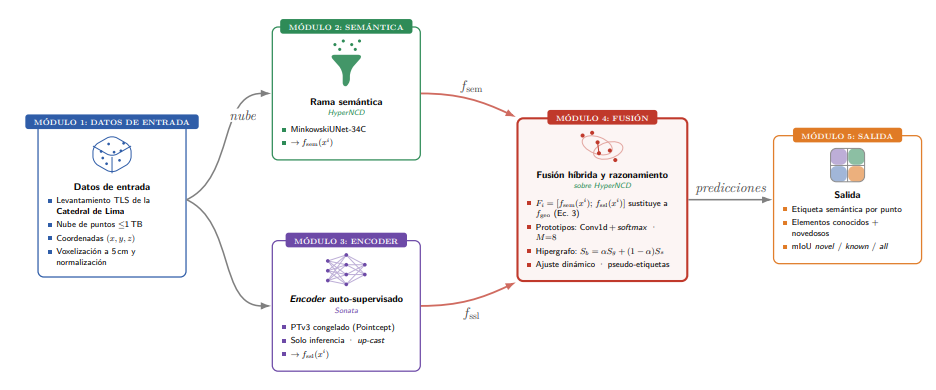
\includegraphics[width=\linewidth]{imagenes/grafico.png}
\caption{Diagrama de diseño del sistema propuesto. La nube TLS de la Catedral de
Lima (Módulo~1) alimenta en paralelo dos ramas de extracción: la rama semántica
MinkowskiUNet-34C de HyperNCD (Módulo~2), que produce $f_{\mathrm{sem}}$, y el
\emph{encoder} PTv3 preentrenado de Sonata (Módulo~3), congelado y usado solo en
inferencia, que produce $f_{\mathrm{ssl}}$. Ambos descriptores entran al
Módulo~4, donde reside el aporte de la tesis: la concatenación
$F_i=[f_{\mathrm{sem}}(x^i);f_{\mathrm{ssl}}(x^i)]$ reemplaza al descriptor
geométrico manual $f_{\mathrm{geo}}$ antes de la formación de prototipos y del
razonamiento por hipergrafo, que permanecen intactos, de modo que la variación de
la métrica sea atribuible al reemplazo.}
\label{fig:diseno}
\end{figure}

El \textbf{Bloque~1} es HyperNCD: aporta la rama semántica (MinkowskiUNet-34C) y
toda la maquinaria de prototipos, hipergrafo dinámico y pseudo-etiquetas que
permite descubrir clases nuevas. El \textbf{Bloque~2} es Sonata: un
\emph{encoder} PTv3 preentrenado de forma auto-supervisada, usado con pesos
congelados y solo en inferencia. El \textbf{nodo de fusión} es el aporte de la
tesis: allí, y solo allí, se sustituye $f_{\mathrm{geo}}$ por $f_{\mathrm{ssl}}$
antes de la formación de prototipos.

\section{Punto de fusión y trazabilidad de la métrica}

Al mover una sola pieza, cualquier variación de la métrica es atribuible al
reemplazo, lo que hace la ablación interpretable sin ambigüedad. Aguas abajo de
la fusión, la afinidad entre prototipos sigue combinando componente geométrica y
semántica según la Ec.~\eqref{eq:afinidad}, y cada prototipo conserva sus $M=8$
vecinos al construir el hipergrafo.

Como el \emph{pipeline} es separable en dos etapas ---inferencia congelada de
Sonata y luego razonamiento de HyperNCD---, la métrica se reporta también en el
punto intermedio y no solo al final: \emph{linear probing} sobre el descriptor
antes de la formación de prototipos (Ec.~\eqref{eq:probe}) y mIoU después
(Ec.~\eqref{eq:miou}). Esa separación es la que permite atribuir una mejora a la
representación o al razonamiento (Sección~\ref{sec:metricas-hibrido}).

\section{Procedimiento experimental}

El procedimiento se ejecuta en cuatro pasos reproducibles. El primero es insumo
de la revisión crítica; los tres restantes corresponden a los objetivos
específicos.

\begin{enumerate}
\item \textbf{Preparación y línea base (Módulo~1).} Teselado de la nube en cinco
secciones disjuntas, voxelización a 5\,cm y normalización; ejecución de HyperNCD
sin modificaciones con tres semillas distintas para fijar el punto de partida de
la Tabla~\ref{tab:base}. El cambio de esquema de normalización fue ensayado y
descartado como resultado negativo (Sección~\ref{sec:linea-base}).
\item \textbf{Fusión (OE1).} Inferencia congelada de Sonata sobre cada sección,
con \emph{cache} de características y \emph{up-cast} para conciliar la resolución
del \emph{encoder} PTv3 con la rejilla de Minkowski; sustitución del descriptor
según la Ec.~\eqref{eq:hibrido} y verificación de funcionamiento de extremo a
extremo sobre una sección de control.
\item \textbf{Calibración (OE2).} Búsqueda por grilla acotada sobre $\alpha$, $M$
y $\epsilon$ en la sección de referencia; la configuración ganadora se congela y
se aplica sin reajuste al resto de secciones.
\item \textbf{Análisis (OE3).} Cómputo de $\Delta$mIoU \emph{novel}
(Ec.~\eqref{eq:delta}), de la brecha cerrada $G$ (Ec.~\eqref{eq:G}) y del
análisis de dominancia (Ec.~\eqref{eq:dominante}), más la ablación de las tres
variantes del descriptor.
\end{enumerate}

\section{Ventaja de dominio del objeto de estudio}

Sonata se preentrenó sobre escenas interiores densas (ScanNet, S3DIS,
Structured3D, HM3D). En LiDAR urbano exterior su \emph{linear probing} queda por
debajo de PTv3 entrenado desde cero (62,0 frente a 69,1 mIoU en SemanticKITTI),
pero en interiores arquitectónicos densos alcanza 72,5 mIoU en ScanNet y 72,3 en
S3DIS Área~5, a la par de modelos supervisados completos. El levantamiento de una
catedral ---estático, denso, de geometría arquitectónica--- cae del lado
favorable de esa frontera, lo que reduce sustancialmente el principal riesgo de
transferencia de dominio.

\section{Riesgos y mitigación}
\label{sec:riesgos}

\paragraph*{(i) Disponibilidad de la nube anotada.} NCD exige al menos las clases
conocidas etiquetadas. Se asume la anotación manual de una sección de referencia
con $\geq$4 clases base; si el levantamiento llega sin etiquetas, esa anotación
se vuelve tarea previa del cronograma y condiciona el inicio de OE1.

\paragraph*{(ii) Acceso y configuración del clúster.} La configuración de GPU de
Khipu ha cambiado respecto de la documentada previamente. Por ello el proyecto no
estima tiempos de calendario: verifica empíricamente el hardware asignado
(Tabla~\ref{tab:hardware}) y fija a partir de esa verificación el tamaño de
ventana y el esquema de \emph{cache}. El seccionamiento de la catedral es el
mecanismo que sostiene el respaldo: ninguna etapa requiere la nube completa en
memoria.

\paragraph*{(iii) Sustitución frente a concatenación (Plan~B).} Si el reemplazo
directo degrada el rendimiento, la variante es concatenar
$F_i=[f_{\mathrm{sem}};f_{\mathrm{geo}};f_{\mathrm{ssl}}]$, dejando que el módulo
de prototipos pondere las tres fuentes. Cualquier resultado ---mejora, paridad o
degradación--- documentado con ablación es reportable.

%%\chapter{RESULTADOS}
\label{cap:resultados}

\section{Experimentos y Resultados}

Los resultados se organizan según los objetivos específicos: \textbf{dos
resultados computacionales} (OE1 y OE2) y una \textbf{salida analítica} (OE3) que
los integra. El punto de partida contra el que se comparan es la línea base
reproducida en la Sección~\ref{sec:linea-base}.

\subsection{Resultado de OE1: modelo híbrido funcional}

Un modelo híbrido verificado de extremo a extremo sobre una sección de control:
la sustitución de $f_{\mathrm{geo}}$ por $f_{\mathrm{ssl}}$ opera dentro del
módulo de prototipos sin romper el razonamiento por hipergrafo y sin degradar el
mIoU \emph{known} respecto de la línea base de la Tabla~\ref{tab:base}. El
entregable incluye la \emph{prueba de funcionamiento} y no solo el código:
inferencia completa, dimensiones documentadas de ambas ramas y verificación de la
compatibilidad de resolución entre el \emph{encoder} PTv3 y la rejilla de
Minkowski.

\subsection{Resultado de OE2: configuración calibrada}

Curvas de sensibilidad de $\alpha$, $M$ y $\epsilon$ sobre la sección de
referencia y una configuración fijada que se aplica sin reajuste al resto de
secciones (Tabla~\ref{tab:sensibilidad}). La lectura esperada es identificar cuál
de los tres parámetros domina el comportamiento del híbrido; en particular, el
valor de $\alpha$ que maximiza el mIoU \emph{novel} indica cuánto peso conserva
la componente geométrica una vez que el descriptor manual ha sido reemplazado.

\begin{table}[H]
\centering
\caption{Sensibilidad de la configuración del híbrido sobre la sección de
referencia.}
\label{tab:sensibilidad}
\begin{tabular}{@{}lccc@{}}
\toprule
\textbf{Parámetro} & \textbf{Rango explorado} & \textbf{Valor fijado} & \textbf{mIoU \emph{novel}} \\
\midrule
$\alpha$   & $[0,\,1]$            & --- & --- \\
$M$        & $\{4,\,8,\,16\}$     & --- & --- \\
$\epsilon$ & \emph{[por definir]} & --- & --- \\
\bottomrule
\end{tabular}
\end{table}

\subsection{Salida analítica de OE3: comparación y ablación}

El resultado central es un incremento medible del mIoU sobre las clases novedosas
respecto de HyperNCD sin modificar, sin degradación de las clases conocidas. La
Tabla~\ref{tab:comparativa} organiza la comparación y la ablación de las tres
variantes del descriptor, aislando la contribución del \emph{encoder}.

\begin{table}[H]
\centering
\caption{Comparación y ablación de las tres variantes del descriptor. Cada fila
reporta además el vector completo de IoU por clase, no solo el agregado
(Sección~\ref{sec:metricas}).}
\label{tab:comparativa}
\begin{tabular}{@{}lcccc@{}}
\toprule
\textbf{Variante del descriptor} & \textbf{mIoU \emph{novel}} & \textbf{mIoU \emph{known}} & $\Delta$\textbf{mIoU} & $G$ \\
\midrule
$[f_{\mathrm{sem}};f_{\mathrm{geo}}]$ (línea base) & --- & --- & --- & 0 \\
$[f_{\mathrm{sem}};f_{\mathrm{ssl}}]$ (propuesto) & --- & --- & --- & --- \\
$[f_{\mathrm{sem}};f_{\mathrm{geo}};f_{\mathrm{ssl}}]$ (Plan~B) & --- & --- & --- & --- \\
\bottomrule
\end{tabular}
\end{table}

\subsection{Entregables}

\begin{enumerate}
\item Línea base reproducida con desviación estándar reportada y análisis de sus
causas, junto con el resultado negativo del Módulo~1
(Sección~\ref{sec:linea-base}).
\item Implementación del modelo híbrido, con prueba de funcionamiento y
repositorio público (OE1).
\item Curvas de sensibilidad de $\alpha$, $M$ y $\epsilon$ y configuración fijada
(OE2).
\item Tablas comparativas, ablación de tres variantes, valores de $G$ y frontera
de operación declarada (OE3).
\end{enumerate}

\section{Discusión}

\paragraph*{Lectura de la métrica.} Un valor de $G$ (Ec.~\eqref{eq:G}) no se
reporta solo. Se acompaña de los tres términos que lo componen y del análisis de
dominancia de la Ec.~\eqref{eq:dominante}: qué clase concreta explica el agregado
y si la ganancia es homogénea entre secciones o está concentrada en una tipología
de elemento. Una mejora que provenga de una sola clase abundante no es el mismo
resultado que una mejora repartida, aunque el mIoU coincida.

\paragraph*{Atribución.} La comparación del \emph{linear probing}
(Ec.~\eqref{eq:probe}) antes de la formación de prototipos con el mIoU final
determina si la ganancia se origina en la representación o en el razonamiento por
hipergrafo. Esa separación es posible porque el \emph{pipeline} es secuencial; si
el sistema fuese unificado, habría que discutir la adecuación misma de la métrica
elegida antes de interpretar el resultado.

\paragraph*{Frontera de operación.} Barriendo densidad de puntos, tamaño de
sección y número de clases novedosas se determina empíricamente la frontera entre
el rango favorable y el desfavorable declarados en el alcance, y se contrasta con
el comportamiento observado en la línea base.

\paragraph*{Realimentación.} Si el análisis muestra que la mejora no se sostiene,
el ajuste se realiza sobre OE1 (esquema de fusión) y OE2 (calibración), no sobre
este capítulo: OE3 es salida analítica y no trabajo computacional independiente.

\paragraph*{Valor para el usuario.} Cada punto de mIoU adicional sobre clases
novedosas es trabajo manual de corrección que deja de realizarse. Los usuarios
están conformes con la precisión que obtienen hoy por vía manual, de modo que la
propuesta de valor no es igualarla sino automatizarla a una precisión suficiente;
sin mejora demostrada sobre el estado del arte, la herramienta no tiene caso.

\paragraph*{Contribución esperada al estado del arte.} La contribución no es una
arquitectura nueva, sino establecer si un hallazgo demostrado en régimen
supervisado ---la nocividad del \emph{geometric shortcut}--- se transfiere al
régimen de descubrimiento de clases novedosas, donde la calidad de la
representación es más crítica porque no hay supervisión sobre las clases
objetivo. Bajo el Plan~B descrito en la Sección~\ref{sec:riesgos}, incluso un
resultado nulo o negativo, documentado con ablación, constituye un hallazgo
reportable.

%%\customchapter{CONCLUSIONES}

Las conclusiones se enuncian en correspondencia con los dos objetivos específicos
que incorporan trabajo computacional, precedidas del diagnóstico que fundamenta
el proyecto y seguidas de la lectura analítica que los integra.

\begin{enumerate}
\item \textbf{Diagnóstico.} La clasificación de elementos estructurales sobre
levantamientos TLS de patrimonio arquitectónico carece hoy de solución
automatizada. La segmentación semántica 3D de conjunto cerrado no puede cubrirla
porque fuerza todo elemento no previsto hacia una clase conocida, y el marco que
sí levanta ese supuesto ---NCD--- rinde entre 11,8 y 47,5 mIoU en clases
novedosas, por debajo del umbral de utilidad práctica. La revisión crítica
localiza la causa plausible en el descriptor geométrico calculado a mano del
módulo de prototipos, y la reproducción de la línea base
(Sección~\ref{sec:linea-base}) fija el punto de partida sobre datos reales, con
el resultado negativo del cambio de normalización descartando una explicación
alternativa.

\item \textbf{Conclusión asociada a OE1 (integración).} La sustitución de
$f_{\mathrm{geo}}$ por la representación auto-supervisada congelada
$f_{\mathrm{ssl}}$ es \emph{[viable / viable bajo condiciones / no viable]}
dentro del módulo de prototipos de HyperNCD, conservando intacto el razonamiento
por hipergrafo. La compatibilidad de resolución entre el \emph{encoder} PTv3 y la
rejilla de Minkowski se resuelve mediante \emph{up-cast} y \emph{cache} por
sección, y la prueba de funcionamiento sobre la sección de control confirma que
el mIoU \emph{known} no se degrada respecto de la línea base.

\item \textbf{Conclusión asociada a OE2 (calibración del híbrido).} El parámetro
que domina el comportamiento del modelo combinado es \emph{[por determinar]}; el
valor de $\alpha$ que maximiza el mIoU \emph{novel} indica cuánto peso conserva
la componente geométrica una vez reemplazado el descriptor manual. La atribución
por etapas muestra que la ganancia se origina principalmente en \emph{[la
representación / el razonamiento por hipergrafo]}, resultado que no sería
observable si el híbrido se evaluara como caja negra.

\item \textbf{Lectura integrada (OE3).} La mejora se cuantifica mediante
$\Delta$mIoU \emph{novel} y la brecha cerrada $G$, reportando siempre los tres
términos que componen esa métrica y la clase que domina el agregado. El diseño
aísla el reemplazo en un único punto de fusión, lo que hace que cualquier
variación de la métrica sea atribuible al cambio y convierte el estudio de
ablación en la evidencia central del trabajo.

\item \textbf{Alcance y límites.} El estudio se realiza sobre un edificio
nombrado y un levantamiento de $\sim$1--2\,GB organizado en cinco secciones, con
rangos de operación declarados por adelantado y verificados empíricamente. El
proyecto está limitado por cómputo y su ejecución depende del hardware
efectivamente asignado en el clúster Khipu, cuya configuración se verifica y no
se estima, lo que hace el proyecto ejecutable con los recursos disponibles y
verificable en sus límites.
\end{enumerate}

%%\customchapter{TRABAJOS FUTUROS}

\begin{itemize}
\item \textbf{Extensión a otras tipologías patrimoniales.} Validar el modelo
híbrido sobre edificaciones de tipología distinta a la de catedral colonial
(conventos, huacas, arquitectura republicana) para medir la pérdida de
rendimiento fuera de la generalización declarada.

\item \textbf{Segmentación de instancias.} Pasar del etiquetado por punto a la
individualización de elementos (columna~1, columna~2), requisito para la
generación automática del modelo BIM.

\item \textbf{Ornamento fino.} Explorar esquemas de resolución adaptativa que
levanten la limitación del vóxel de 5\,cm sobre elementos decorativos por debajo
de esa escala.

\item \textbf{Preentrenamiento específico de dominio.} Evaluar si un
preentrenamiento auto-supervisado sobre un corpus de levantamientos
patrimoniales mejora las representaciones respecto de los pesos públicos de
Sonata, entrenados sobre escenas interiores genéricas.

\item \textbf{Vocabulario abierto.} Integrar modelos de lenguaje-visión para
nombrar automáticamente las clases descubiertas, en lugar de dejarlas como
agrupaciones sin etiqueta semántica.
\end{itemize}
 % sección opcional

%% ============================================================================
\renewcommand{\bibname}{\hfill\Large\bf{REFERENCIAS BIBLIOGRÁFICAS}\hfill}

\bibliographystyle{IEEEtran} % Estableciendo el estilo de citas IEEEtram.

\bibliography{referencias} % Recibe las referencias de IEEE

\appendix
\customchapter{ANEXOS}

\section*{Anexo A. Configuración de \emph{software}}

Python 3.10, PyTorch, MinkowskiEngine, \texttt{spconv}, Pointcept, código oficial
de HyperNCD y pesos públicos de Sonata. Seguimiento de experimentos con
Weights~\&~Biases.

\section*{Anexo B. Nomenclatura}

\begin{tabular}{@{}ll@{}}
\toprule
\textbf{Símbolo} & \textbf{Significado} \\
\midrule
$P$ & Nube de puntos del levantamiento \\
$\mathcal{C}_k$ & Conjunto de clases conocidas (etiquetadas) \\
$\mathcal{C}_n$ & Conjunto de clases novedosas (sin etiqueta) \\
$f_{\mathrm{sem}}$ & Descriptor semántico (MinkowskiUNet-34C) \\
$f_{\mathrm{geo}}$ & Descriptor geométrico calculado a mano \\
$f_{\mathrm{ssl}}$ & Descriptor auto-supervisado (Sonata, congelado) \\
$\alpha$ & Balance geométrico-semántico en la afinidad $S_b$ \\
$M$ & Vecinos por hiperarista \\
$\epsilon$ & Suavizado de etiquetas \\
\bottomrule
\end{tabular}


\end{document}
